\documentclass[12pt,a4paper]{article}
\usepackage[utf8]{inputenc}
\usepackage[a4paper,vmargin={17mm,20mm},hmargin={20mm,10mm}]{geometry}
\usepackage{amsmath}
\usepackage{amssymb}
\usepackage{mathtools}
\usepackage{gensymb}
\usepackage{enumitem}
\usepackage{graphicx}
\usepackage{scrextend}
\usepackage{blindtext}
\usepackage{caption}
\usepackage{url}
\usepackage{subcaption}
\usepackage{circuitikz}
\usepackage{listings}
\usepackage{color}
\usepackage{hyperref}
\usepackage{subcaption}
 
\definecolor{codegreen}{rgb}{0,0.6,0}
\definecolor{codegray}{rgb}{0.5,0.5,0.5}
\definecolor{codepurple}{rgb}{0.58,0,0.82}
\definecolor{backcolour}{rgb}{0.95,0.95,0.92}
 
\lstdefinestyle{mystyle}{
    backgroundcolor=\color{backcolour},   
    commentstyle=\color{codegreen},
    keywordstyle=\color{magenta},
    numberstyle=\tiny\color{codegray},
    stringstyle=\color{codepurple},
    basicstyle=\footnotesize,
    breakatwhitespace=false,         
    breaklines=true,                 
    captionpos=b,                    
    keepspaces=true,                 
    numbers=left,                    
    numbersep=5pt,                  
    showspaces=false,                
    showstringspaces=false,
    showtabs=false,                  
    tabsize=2
}
 
\lstset{style=mystyle}
 

\DeclarePairedDelimiter\floor{\lfloor}{\rfloor}
\title{AI lab Project Report}
\date{\today}
\author{By Alessandro Vecchi}
\sloppy
\begin{document}
\title{\textbf{AI lab Project Report}}
\author{Alessandro Vecchi and Francesco Danese}
\date{\today}
\maketitle

%this is the tenth question

\begin{abstract}

\begin{addmargin}[3em]{1em}
\centering
Throughout the AI Lab course we have learnt many Computer Vision and Deep Learning concepts and we applied almost all of them directly or indirectly in our final lab project. Additionally, having taken away a lot from this course, we aimed to make a project that would challenge us academically and intellectually. For our final project, we made an autonomous lane-following car, built by us, that is also able to stop in front of STOP signals.
\end{addmargin}

\end{abstract}

\section{Introduction}
%starting off with the answer
\begin{large}
It's been quite a journey. We decided to tackle the problem of building from start to finish a self-driving car with Raspberry Pi 4 with a lane following algorithm that doesn't rely on deep learning, but only on a pipeline of various Image Processing techniques. It's been an awesome project, even if we spent a lot of time doing it we enjoyed every part of it. The feeling of succedingly building a self-driving car is unbearable, not mentioning that it can stop and restart at the STOP signal flawlessly. \\
Originally, we wanted to implement also a lane following algorithm with neural networks and to perform semaphore recognition with a 3D printed semaphore, but we underestimated the amount of time required for this huge project and the rest of the time was spent in internships and for studying the other 4 exams of the semester. But still we manage to complete a lot of tasks and we couldn't be any happier! \\
Next year we could improve the project during the Deep Learning course by creating a neural network solution to the problem and add vocal commands and speech processing tasks during the NLP course. There is still a lot to be done and we can't wait to go further in learning but, for now, let's settle and fully understand the topics of this course!

\newpage
\section{Building the Robot}


\subsection{Components}

The main idea was to build a small car that was able to see. To achieve all the tasks needed for such a robot, we made the following shopping list: 
\begin{itemize}
  \item 3 big batteries for powering the motors (3.7V each one) and a switch.
  \item 1 Powerbank to power the Raspberry.
  \item 4 DC motors and wheels.
  \item A two-level chassis made of plastic plates to accomodate all the devices.
  \item 1 Raspberry-Pi-4 as computational unit, basically, the computer.
  \item 1 L298 h-bridge driver, wired to the batteries and the computer, that takes signals from the Raspberry Output pins and give the right amount of energy to the motors.
  \item 1 Camera of 8MP compatible with the Pi and a Wide-Angle lens to retain a more spreaded view.
  \item A 3D-printed arm to hold the camera lifted up.
  \item A bunch of wirings, double sided tape, screws and bolts.
\end{itemize}
Let's see how those components look: 

\begin{figure}[hb]
  \centering
  \begin{subfigure}{0.2\textwidth}
    \centering
    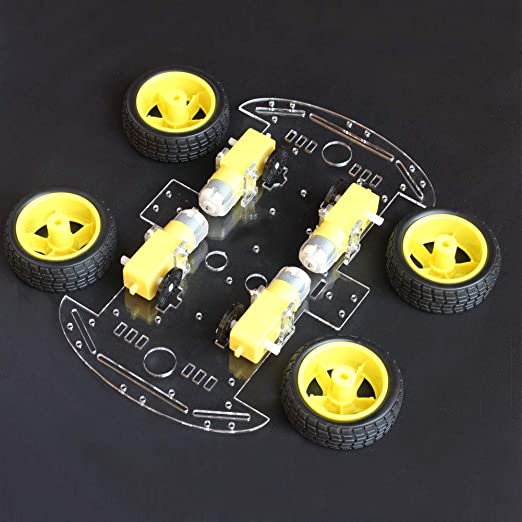
\includegraphics[width = \textwidth]{images/Chassis.jpg}
    \caption{Wheels, motors and chassis}
    \label{fig:left}
    \end{subfigure}
  \begin{subfigure}{0.2\textwidth}
    \centering
    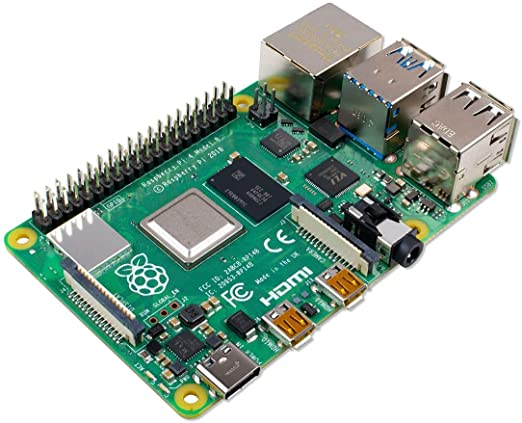
\includegraphics[width = \textwidth]{images/rasp.jpg}
    \caption{Raspberry Pi 4}
    \label{fig:right}
    \end{subfigure}
  \begin{subfigure}{0.2\textwidth}
    \centering
    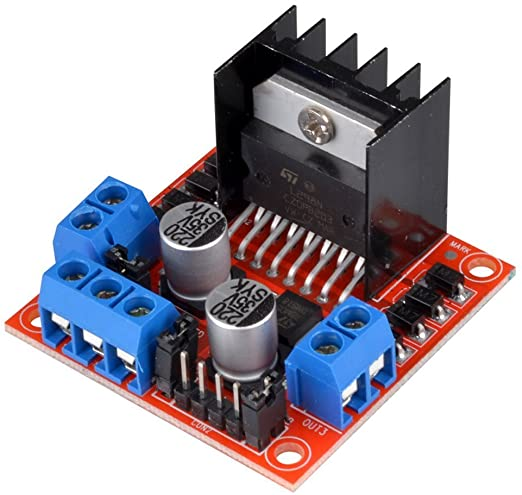
\includegraphics[width = \textwidth]{images/bridge.jpg}
    \caption{L298n Driver}
    \label{fig:right}
    \end{subfigure}
  \begin{subfigure}{0.2\textwidth}
    \centering
    \rotatebox[origin=c]{270}{\includegraphics[width = \textwidth]{images/cameraPi.jpg}}
    \caption{The camera}
    \label{fig:right}
    \end{subfigure}
  \begin{subfigure}{0.2\textwidth}
    \centering
    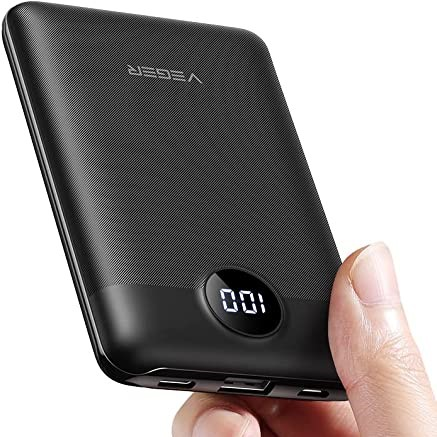
\includegraphics[width = \textwidth]{images/powerbank.jpg}
    \caption{Powerbank}
    \label{fig:right}
    \end{subfigure}
  \begin{subfigure}{0.2\textwidth}
    \centering
    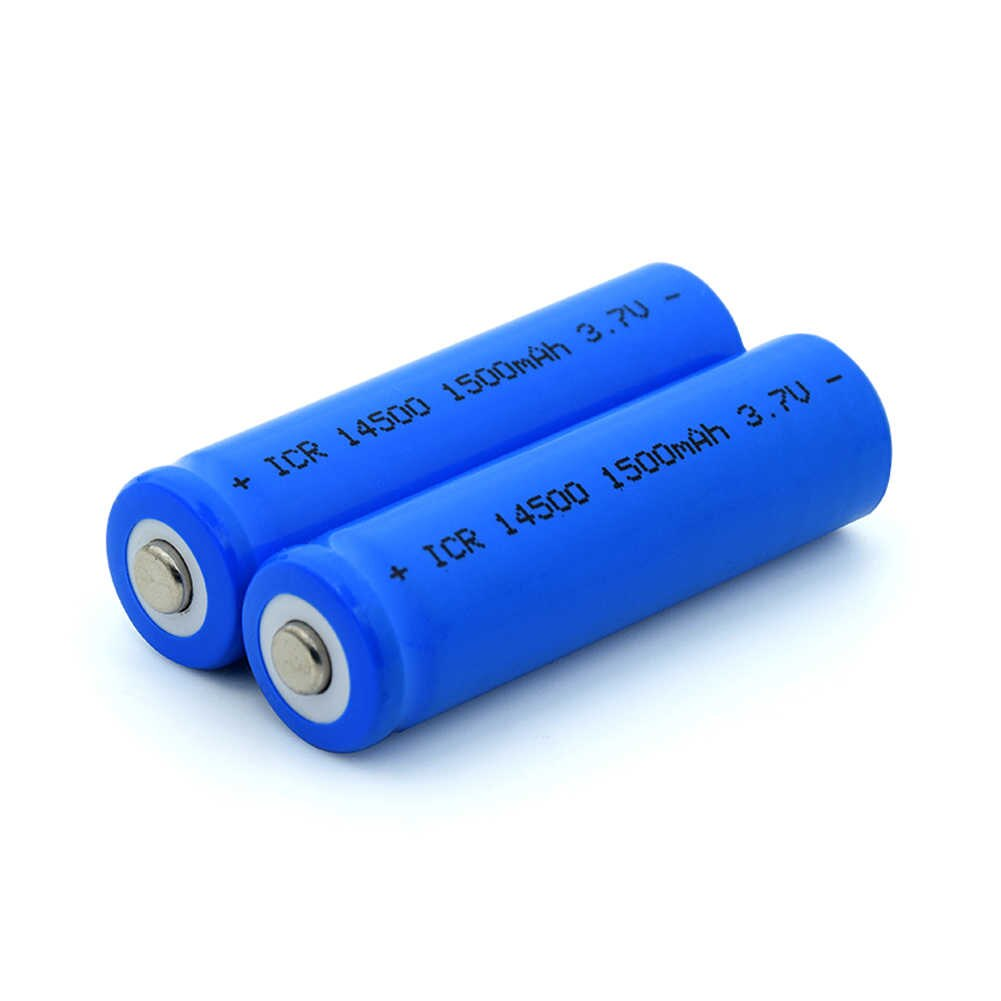
\includegraphics[width = \textwidth]{images/batterie.jpg}
    \caption{Motor's batteries}
    \label{fig:right}
    \end{subfigure}
  \begin{subfigure}{0.2\textwidth}
    \centering
    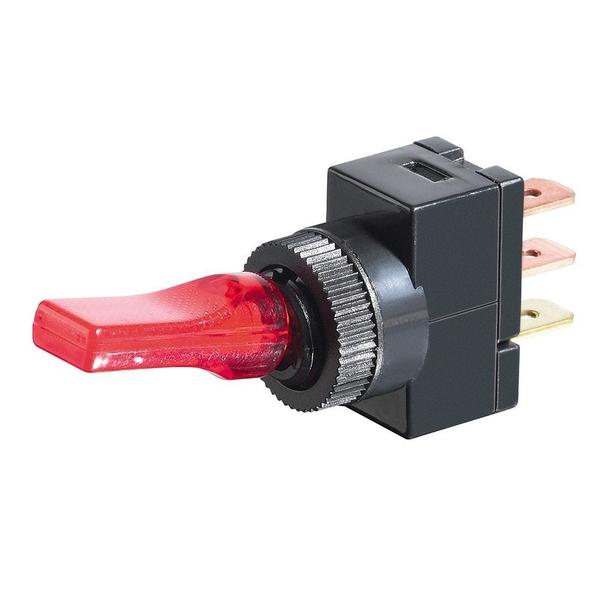
\includegraphics[width = \textwidth]{images/switch.jpg}
    \caption{Power switch}
    \label{fig:right}
    \end{subfigure}
  \label{fig:combined}
\end{figure}

\subsection{Assembling all the parts}
Now it's time to give a sense to this pile of stuff, and mount all the components together. On the bottom level of the robot will be located the two power sources, batteries and powerbank, along with the l298n driver. On the top level will sit the Raspberry and the camera mounted on a 3D-printed support. Here's some pictures of the complete robot:
\begin{figure}[hb]
\centering
\begin{subfigure}{0.32\textwidth}
  \centering
  \rotatebox[origin=c]{270}{\includegraphics[width = \textwidth]{images/robot1.jpg}}
  \label{fig:right}
  \end{subfigure}
\begin{subfigure}{0.32\textwidth}
  \centering
  \rotatebox[origin=c]{270}{\includegraphics[width = \textwidth]{images/robotfront.jpg}}
  \label{fig:right}
  \end{subfigure}
\begin{subfigure}{0.32\textwidth}
  \centering
  \rotatebox[origin=c]{270}{\includegraphics[width = \textwidth]{images/robotside.jpg}}
  \label{fig:right}
  \end{subfigure}
\end{figure}

\subsection{Wirings}

The three blue batteries situated at the bottom level are linked to a switch accessible from below, so that one can turn off/on the power source of the motors whenever needed,useful for saving energy and batteries' lifetime.
The switch is then connected to the l298n Driver, that take as input two 6 cables (3 for pairs of motors, since the ones on the same side have to work in the same way) connected to the rapsberry pi GPIO (General Purpose Input Output) pins.
In the code the 3 cables/pins are refered as "En" "In1" "In2", that stands for Enable, Input One and Input Two. The first is for activation, and the remaining two for deciding the direction, forward or backward.
The raspberry is instead powered by a common smarthpone powerbank, via USB-C cable.
The following is a picture of the wiring schema for the motors: 
\begin{figure}[h!]
  \centering
  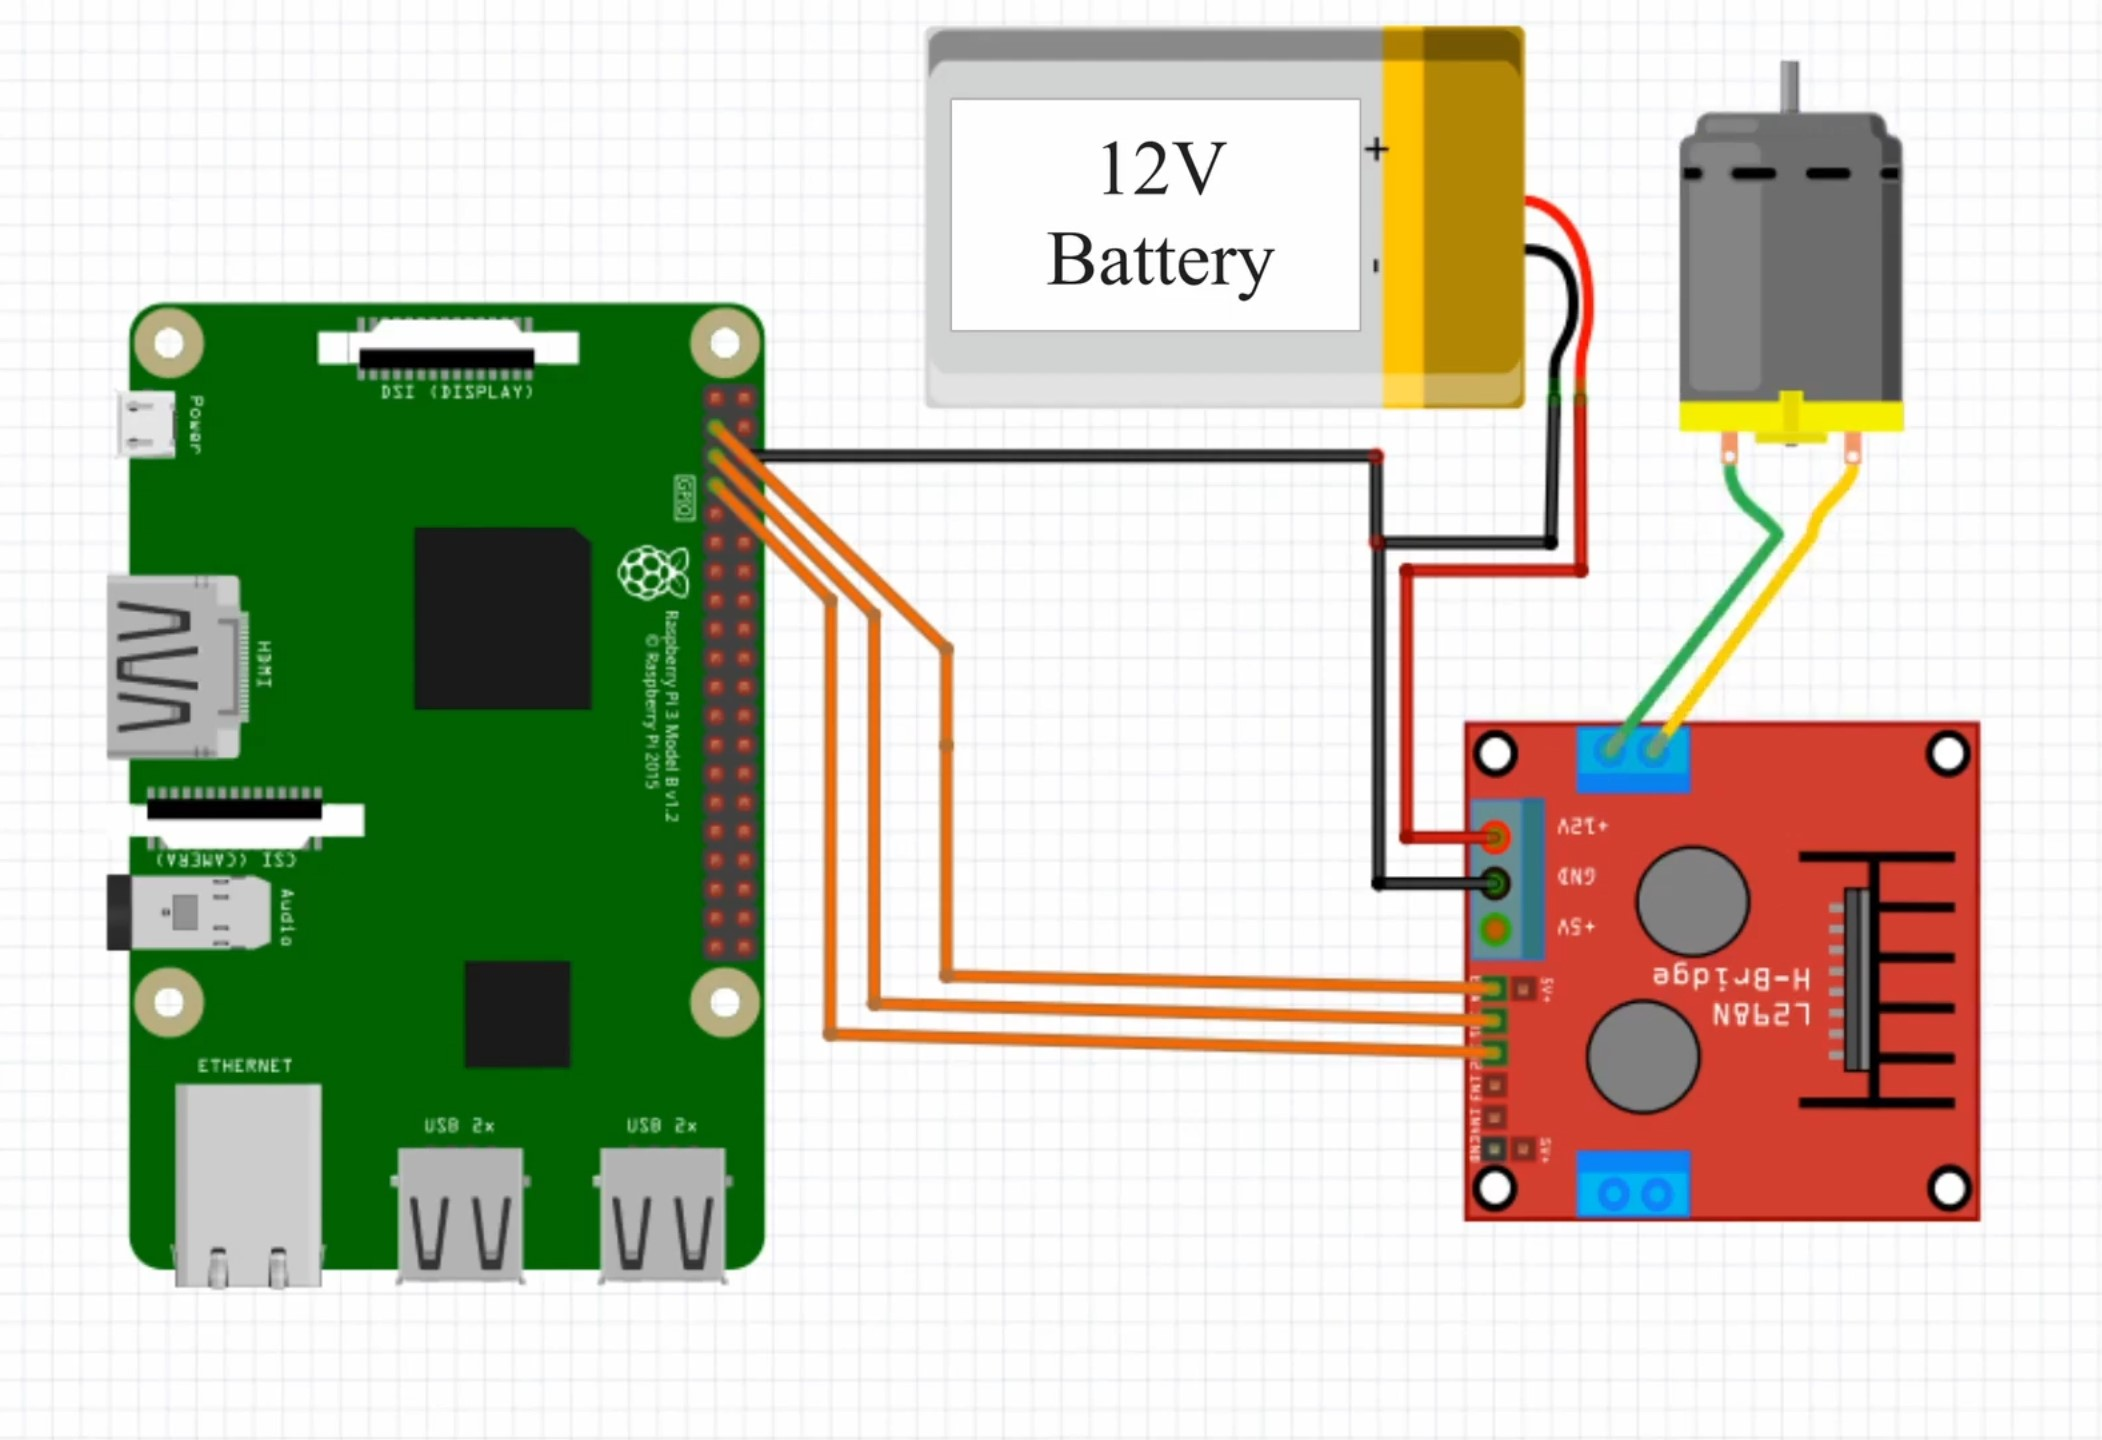
\includegraphics[width = 10cm,height=6cm]{images/schema.jpg}
  \label{fig:schema}
\end{figure}

\subsection{How to Turn}

The wheels can just go forward or backward, no steering device is present. Therefore the car, in order to turn left and right, will apply a difference of speed between right and left side, similarly to tanks and other tracked vehicle.
For istance, if we want to go left, we'll set the speed of the right wheels higher than the speed of the left wheels and viceversa.

\section{Lane detection with Image processing}

The main idea here is to find the path using color detection and then iteratively moving the car at the center of the road.\\
In order to reach this goal we are going to divide the task in 5 different steps:

\begin{itemize}
  \item[1] Thresholding the frames;
  \item[2] Warping the perspective;
  \item[3] Finding the center of the road;
  \item[4] Understanding how to curve;
  \item[5] Hardware implementation.
  \end{itemize}

There are also two small sections that explain how the car recognizes the end of the road and how it makes a U-turn after the first lap.

\begin{figure}[hbp]
\centering
\includegraphics[width=0.6\textwidth, height = 6cm]{images/road.jpg}
\caption{Test track for the vehicle with curved corners}
\end{figure}

\subsection{Thresholding}
Recall that our "street" consists of plain A4 white paper, so a cool way to find the path is to apply simple thresholding to each frame.\\
The original way we were doing it was by converting the BGR image to an HSV one. The reason is that since the hue channel models the color type, it is very useful to segment the road based on its color and we could tune the saturation to express the "whiteness" of our image. Thus to select our path we selected a range of white-ish pixels using trackbars and set them to 255, while all the others were set to 0. However, we then discovered that this method was very dependent to the lightning conditions since it was a static way of determine the threshold and so we had to change the thresholding section a little bit. We tried a lot of methods and the ones that worked best were Otsu's thresholding and a conversion to the HSL color space to remove the very bright portions of the frame.\\
In order to achieve this we will use the \href{https://docs.opencv.org/3.4/da/d97/tutorial_threshold_inRange.html}{inRange} function of OpenCV and to select the right thresholds we use a slightly modified version of the color picker offered by the link above.

\begin{figure} [!htb]
  \centering
    \begin{subfigure}[b]{0.4\textwidth}
    \centering
    \captionsetup{justification=centering}
      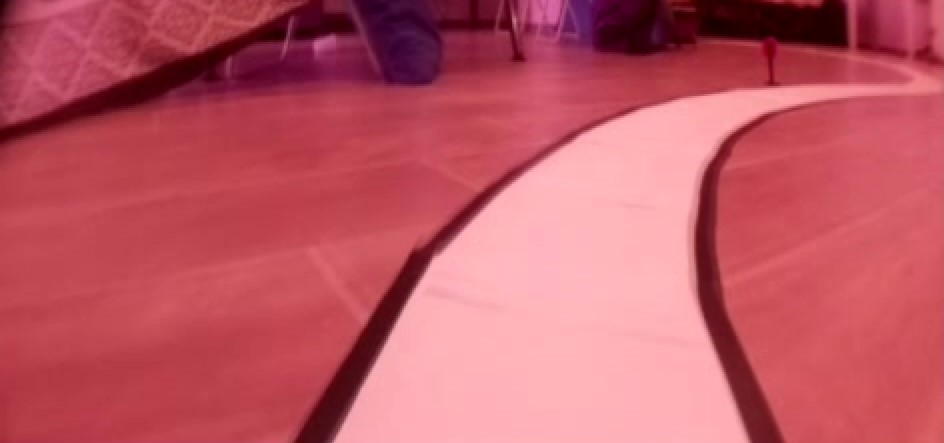
\includegraphics[width=7cm, height = 4.5cm]{images/normal.jpg}
      \caption{How we see the path}
      
    \end{subfigure}
    \hspace{1cm}
    \begin{subfigure}[b]{0.4\textwidth}
    \centering
    \captionsetup{justification=centering}
      
\includegraphics[width= 7cm, height = 4.5cm]{images/thres.jpg}
      \caption{Thresholded path \\}
      
    \end{subfigure}
  \end{figure}

\subsection{Warping}
Recall that one of our goals is to determine the radius of curvature of the road lane, in order to be able to perform the curve. \\
The problem is that the camera perspective is not an accurate representation of what is going on in the real world. From its point of view, the lane lines form a trapezoid-like shape. We can't compute the radius of curvature of the road because the lane width seems converging to a point, as you can see from this example:\\

\begin{figure} [h!]
\centering
\captionsetup{justification=centering}
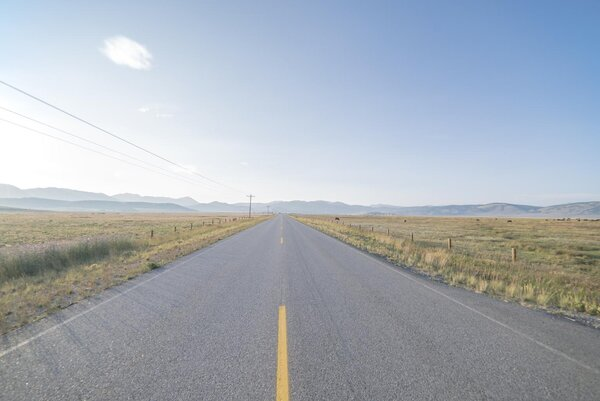
\includegraphics[width=6cm]{images/road_endless_straight_vanishing.jpg}
\caption{Camera's perspective}
\end{figure}

To fix this, we can apply a perspective transformation that warp the camera's perspective into a birds-eye view perspective.

\begin{figure} [h!]
  \centering
  \captionsetup{justification=centering}
  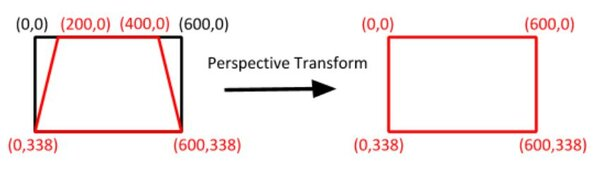
\includegraphics{images/perspective_transform.jpg}
  \caption{Perspective transform}
  \end{figure}

To do this we need to identify the region of interest, defined by the four corner of our trapezoid. In this way we can concentrate only on the parts of the image we're interested in, namely the ones immediately in front of the car. We determined these points manually, by experimenting with different values on the trackbars. Now we can obtain the transformation matrix using the built-in "getPerspectiveTransform"" and then we can get the warped image with the "warpPerspective" method.

\begin{figure} [!hbp]
  \centering
    \begin{subfigure}[b]{0.3\textwidth}
    \centering
    \captionsetup{justification=centering}
      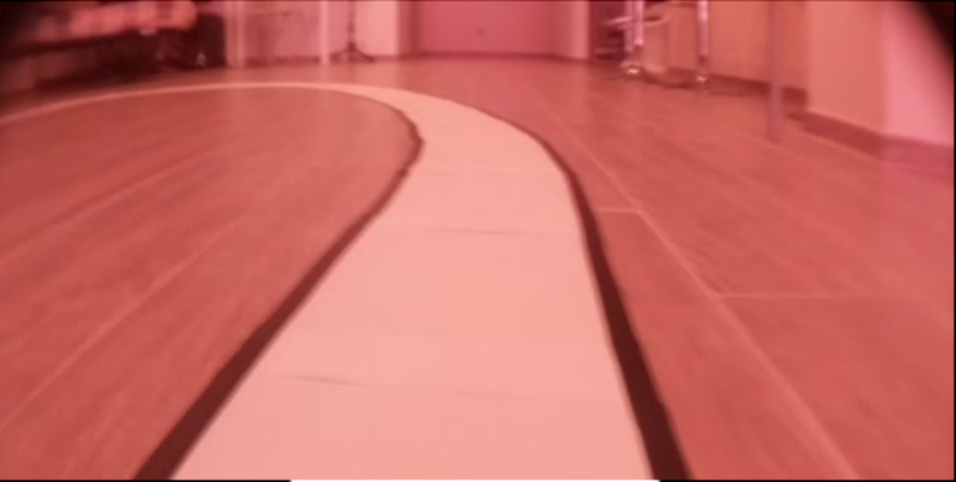
\includegraphics[width=\textwidth]{images/camera_perspective.png}
      \caption{Road in perspective}
      
    \end{subfigure}
    \hspace{0.1cm}
    \begin{subfigure}[b]{0.3\textwidth}
    \centering
    \captionsetup{justification=centering}
      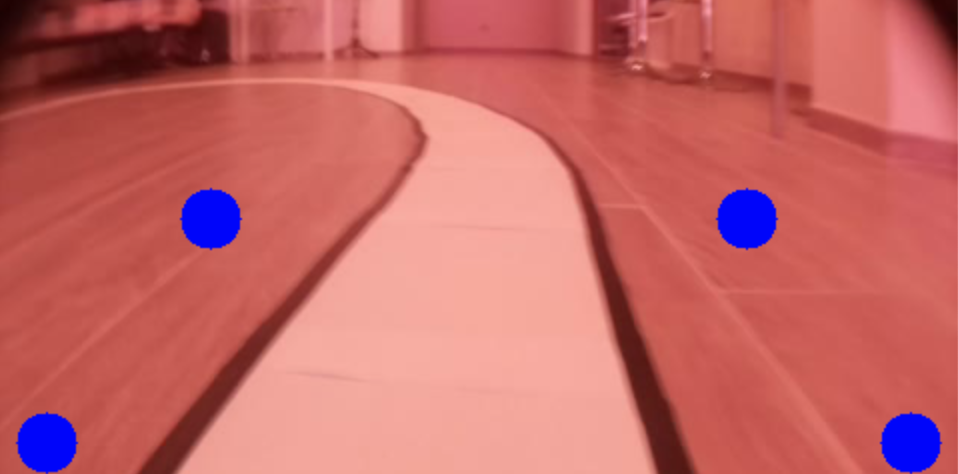
\includegraphics[width=\textwidth]{images/points_warp.png}
      \caption{Points for tuning \\}
      
    \end{subfigure}
    \hspace{0.1cm}
    \begin{subfigure}[b]{0.3\textwidth}
    \centering
    \captionsetup{justification=centering}
      
\includegraphics[width=\textwidth]{images/birds_eye_view.png}
      \caption{Bird eye view \\}
      
    \end{subfigure}
  \end{figure}

\subsection{Centering}
In order for our supercar to move smoothly and to detect curves properly, we have to make it move at the center of the road. But how do we find the center? \\
Well, it turns out that is rather easy. Ideally, we have a black image and a white road seen from above. A logical way of finding the center of the road is to consider the part of the image that is immediately near the camera and find the average column between those that have a relevant amount of white pixels.

\begin{figure} [!htb]
  \centering
  \captionsetup{justification=centering}
  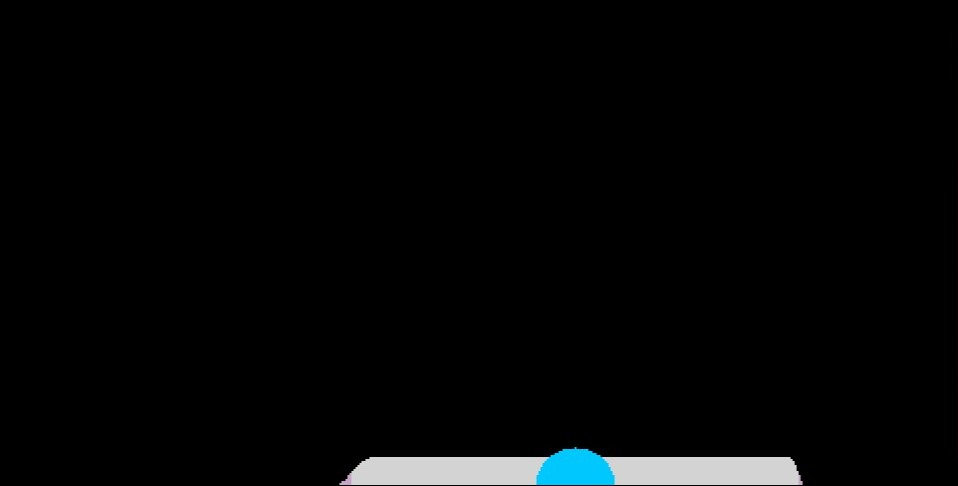
\includegraphics[width=8cm]{images/base.jpg}
  \caption{How the center is determined}
  \end{figure}

\subsection{Finding the radius of curvature}
We're now able to identify the center of the lane properly. We need now to make our car pursue it. Logically enough, the direction the car is going can be represented by the mean column of the image. Since the frame size is $240 \times 480$, the center of the camera is simply $\frac{480}{2}=240$.\\
Therefore, the distance between the road center and the camera center represents the radius of curvature in pixels of the lane. If the center of the street is on the right, than it has to curve right, otherwise left. To avoid useless zig-zag movements, if we are too close to the center we just go straight. \\
Recall that Saetta is powered by motors whose activation is a percentage of the power we want to give to the motors. We determined experimentally that values less than 10\% are bad because the car does not manage to move, while values greater than 60\% are not good because its motors go nuts. 
Thus, we have to find a function that given the distance in pixel between center of the lane and the center of the camera spits as output the speed that have to be added/subtracted to the motor's sides. It is a value more or less between 0.1 and 0.6 that will be add to the current velocity of a side and subtract from the other side. \\
The function we found seems totally out of the blue, so we are going to explain step by step the reasoning we did to find it.
Our goal was to find a function whose radius of curvature was decently high even if the distance from the center was small, but not too high when the distance was large. Moreover, since the distance from the center could also be negative, it had to be symmetric wrt the y axis. Something like this:

\begin{figure} [h!]
  \centering
  \captionsetup{justification=centering}
  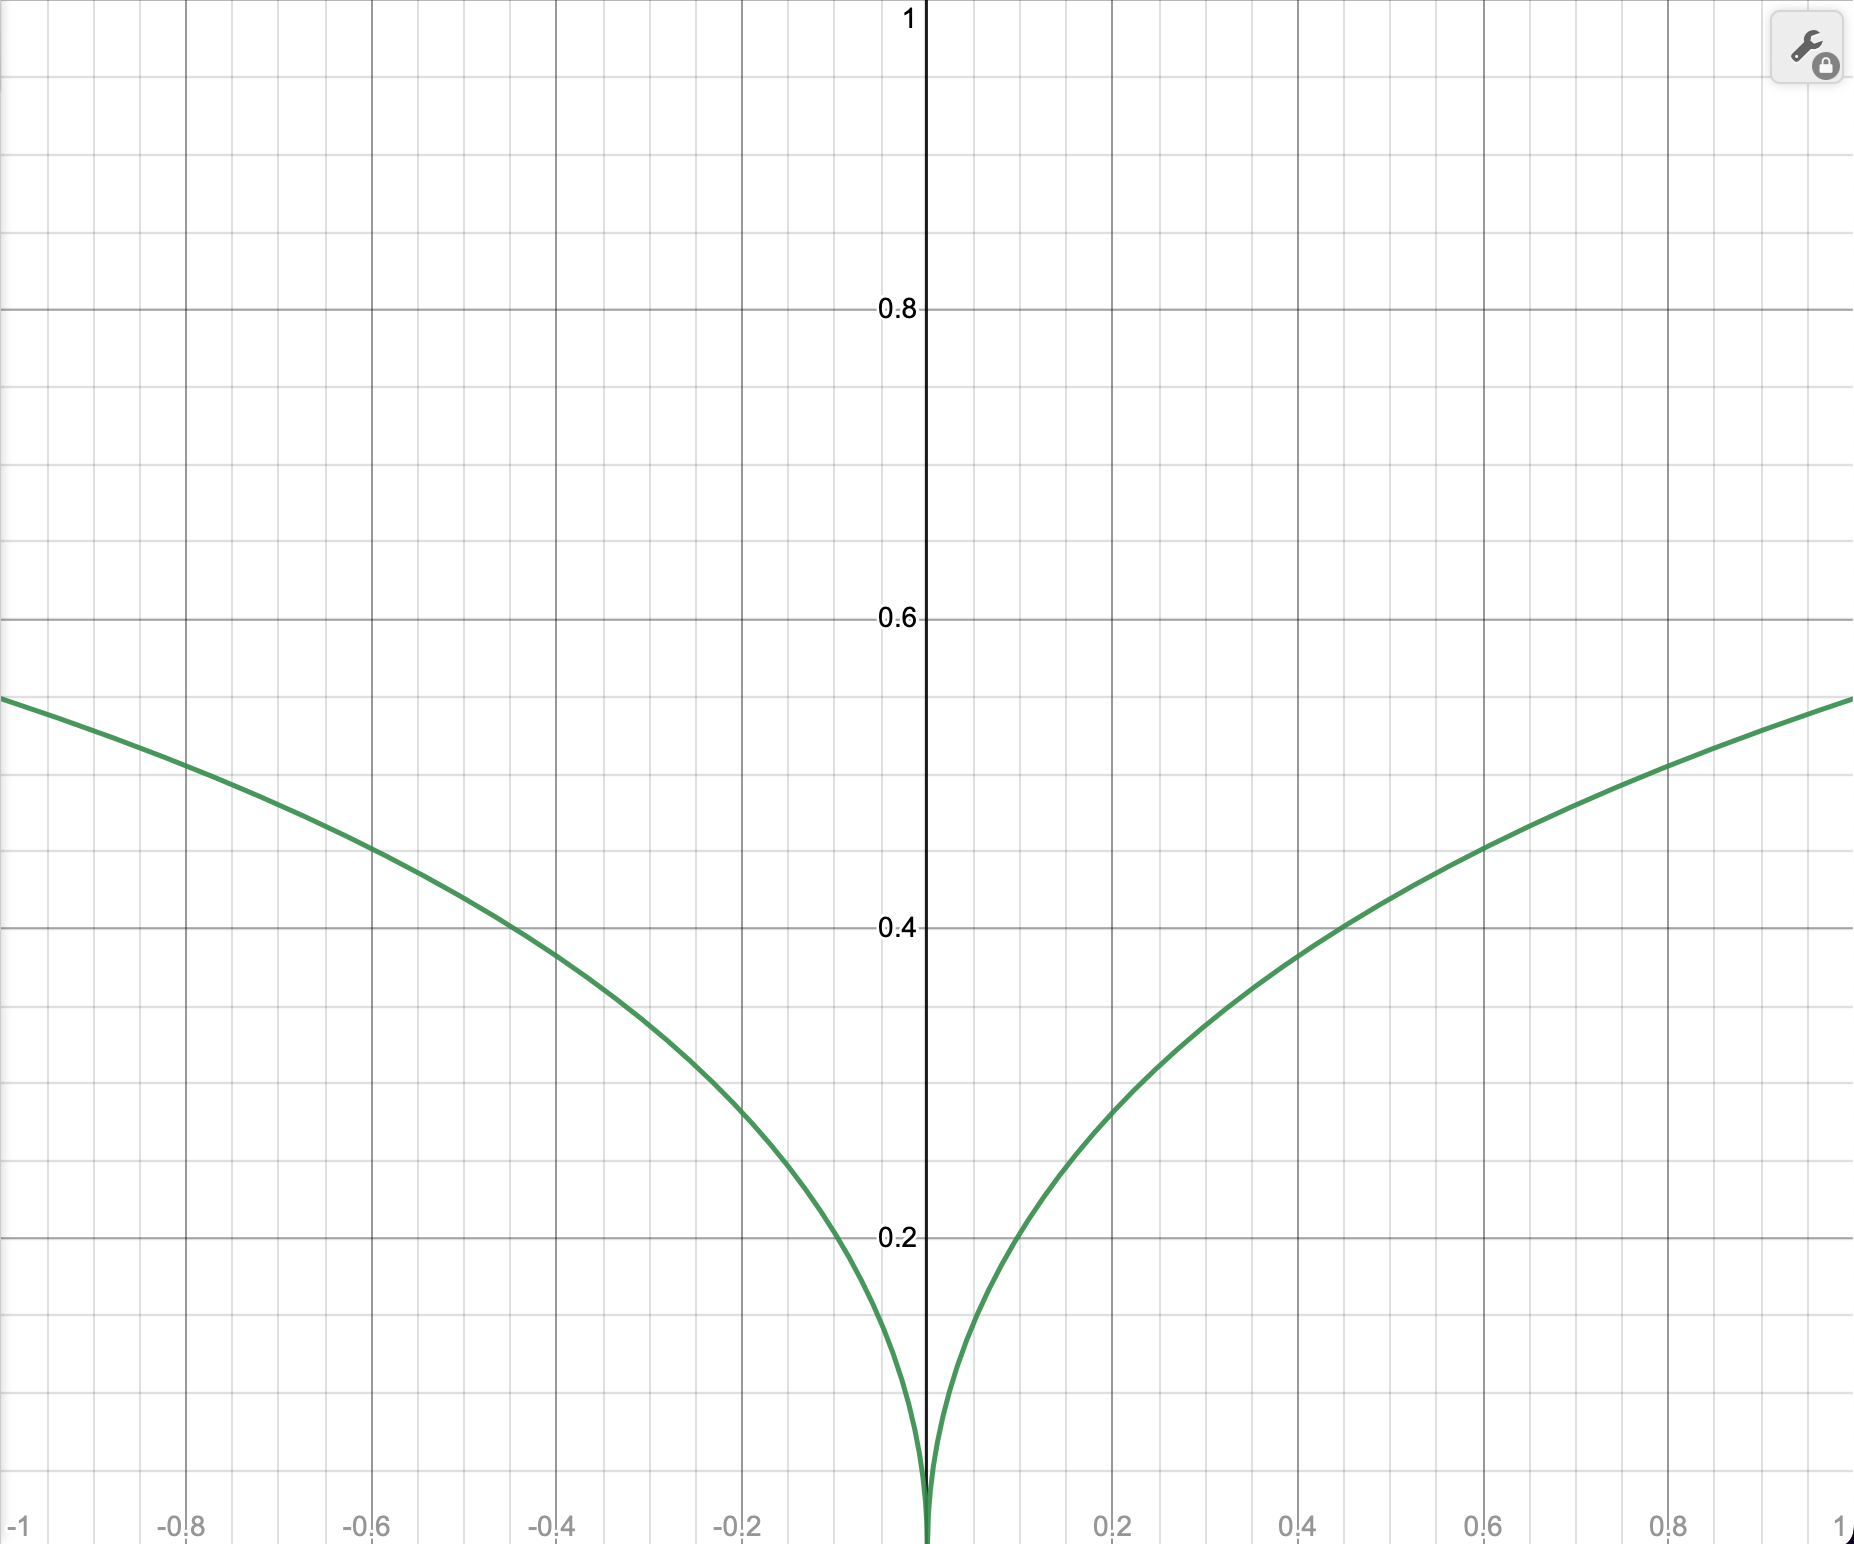
\includegraphics[width=8cm]{images/madFunction.png}
  \caption{Target Function}
  \end{figure}

It has a logarithmic behaviour and it's always positive, so $\log(|x|)$ is a good start. Since want the $x$ to assume values between 0 and 1, we have to normalize the distance by dividing it for 240, because it can take values between 0 and 240. Therefore we have also to add 1 inside the logarithm, otherwise the function will always give negative values.

\begin{figure} [!h]
  \centering
  \captionsetup{justification=centering}
  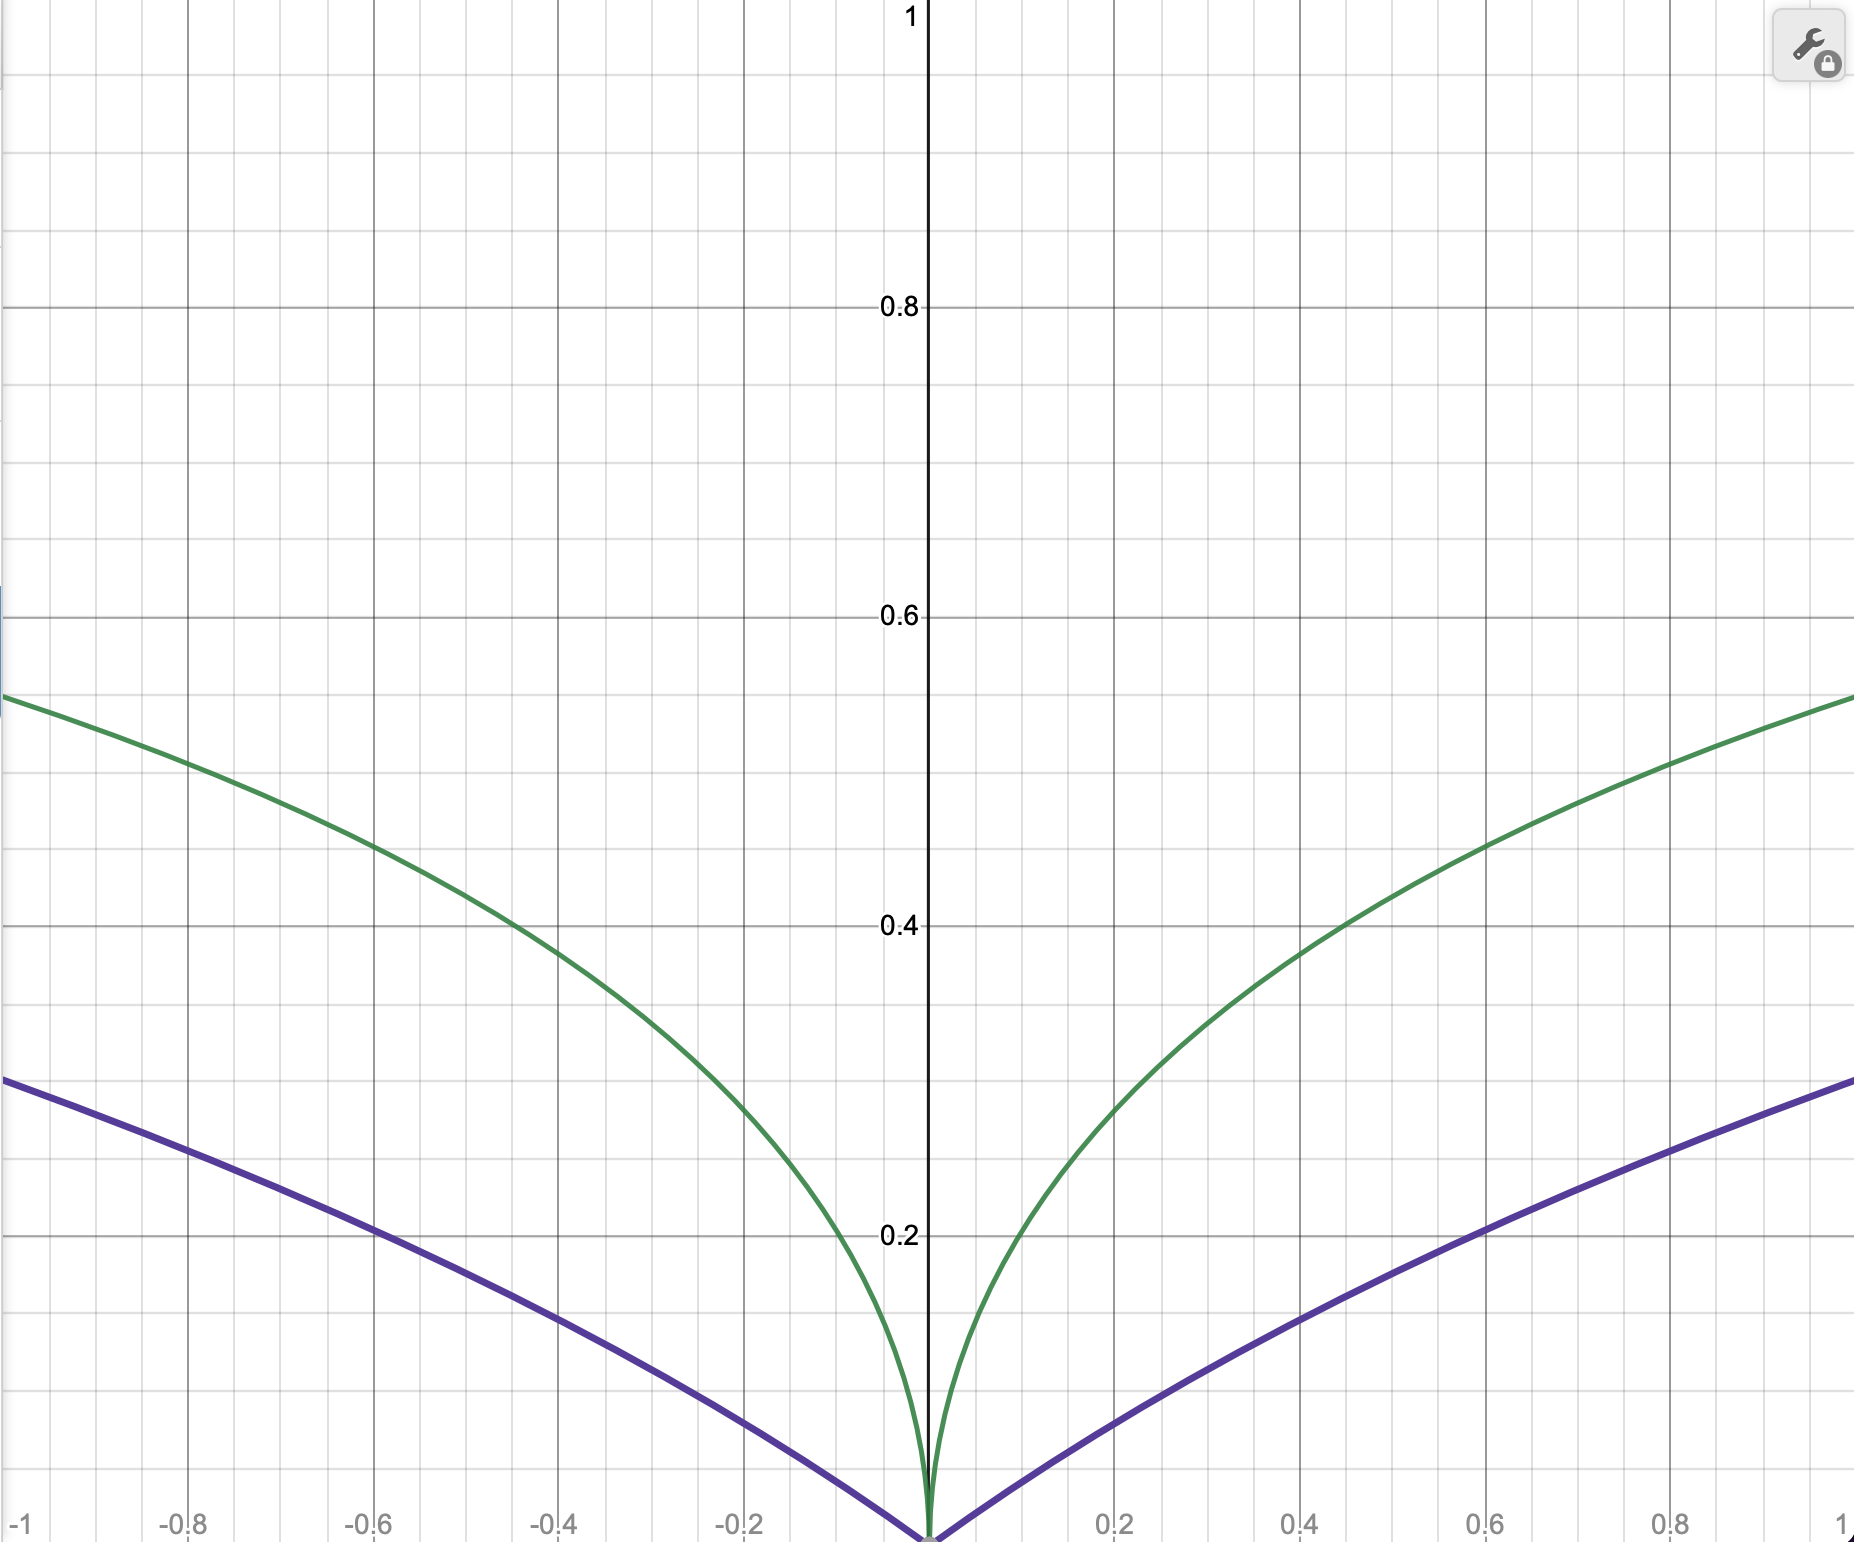
\includegraphics[width=8cm]{images/logx.png}
  \caption{${\color{violet}y=\log(|x|+1)}$ and ${\color{green}y=\sqrt{\log(|x|+1)}}$}
  \end{figure}

As you can see from the graph, its behaviour is too line-shaped to satisfy our goals. Thus we have to pump up the function. Since we are in the 0-1 range, we can't squared it, but we can square root it.
In practice, we also changed the scaling of the $x$ variable because we saw it worked better inside the range between the green and purple function.

\subsection{Hardware implementation}
Now we need to implement the function that acts on the robot.
Simply enough, we're just going to take the smoothed value we just obtained by applying that function and insert it as the parameter by which the car has to curve in the turn module of MotorModule. The velocity will be kept at 0.2 for experimental purposes.

At the end, the whole pipeline looks like this:

\begin{figure} [!hbp]
  \centering
    \begin{subfigure}[b]{0.3\textwidth}
    \centering
    \captionsetup{justification=centering}
      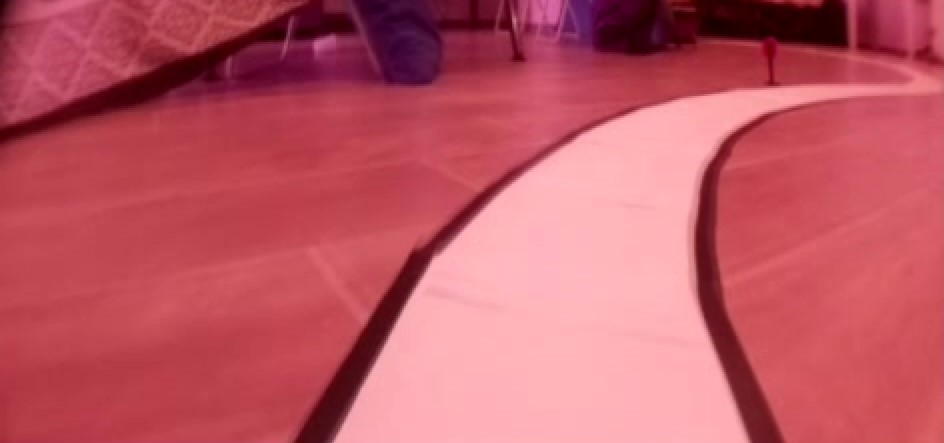
\includegraphics[width=\textwidth]{images/normal.jpg}
      \caption{Road seen from the camera}
      
    \end{subfigure}
    \hspace{0.1cm}
    \begin{subfigure}[b]{0.3\textwidth}
    \centering
    \captionsetup{justification=centering}
      
\includegraphics[width=\textwidth]{images/thres.jpg}
      \caption{Thresholded Image \\}
      
    \end{subfigure}
    \hspace{0.1cm}
    \begin{subfigure}[b]{0.3\textwidth}
    \centering
    \captionsetup{justification=centering}
      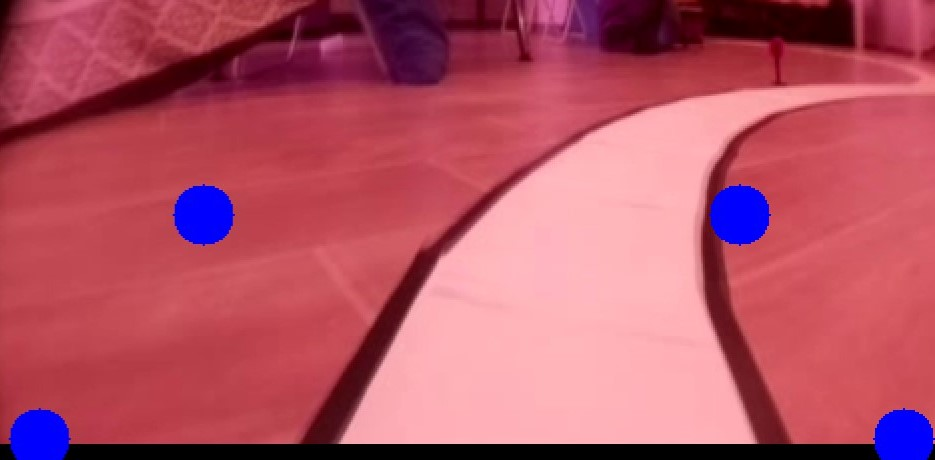
\includegraphics[width=\textwidth]{images/warp.jpg}
      \caption{Points for warping\\}
      
    \end{subfigure}
  \end{figure}

\begin{figure} [!hbp]
  \centering
    \begin{subfigure}[b]{0.3\textwidth}
    \centering
    \captionsetup{justification=centering}
      
\includegraphics[width=\textwidth]{images/warptr.jpg}
      \caption{Bird eye thresholded view}
      
    \end{subfigure}
    \hspace{0.1cm}
    \begin{subfigure}[b]{0.3\textwidth}
    \centering
    \captionsetup{justification=centering}
      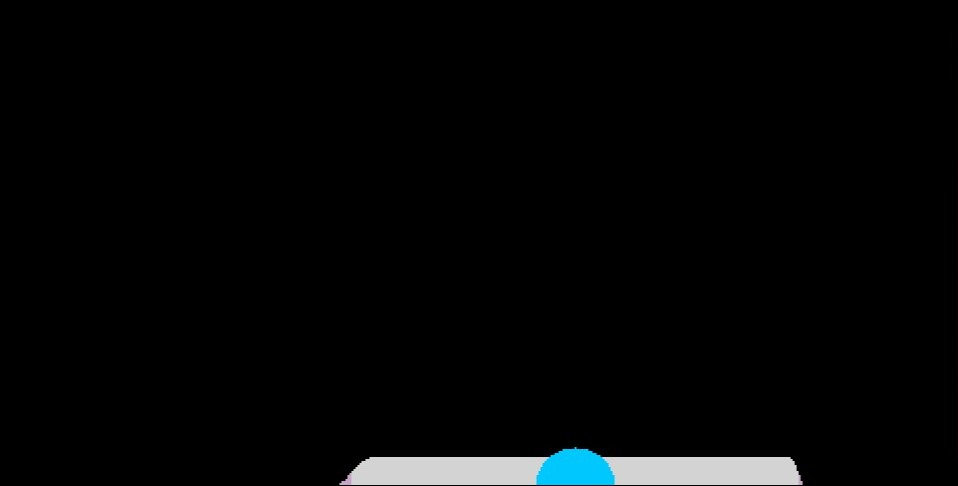
\includegraphics[width=\textwidth]{images/base.jpg}
      \caption{Center of the road \\}
      
    \end{subfigure}
    \hspace{0.1cm}
    \begin{subfigure}[b]{0.3\textwidth}
    \centering
    \captionsetup{justification=centering}
      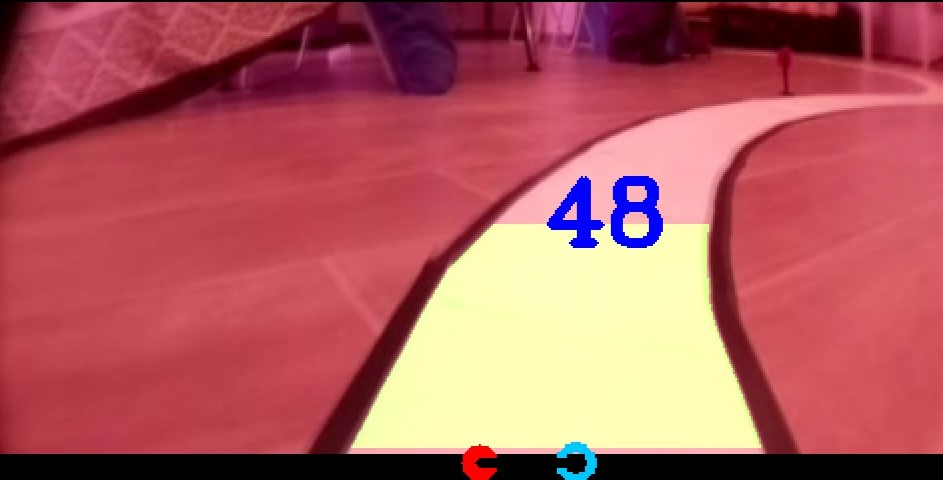
\includegraphics[width=\textwidth]{images/final.jpg}
      \caption{Curve's coefficient  \\}
      
    \end{subfigure}
  \end{figure}
  
\subsection{How to recognize that the lane has ended}
To recognize the end of the track it's enough to just identify a stripe on the mid-bottom part of the warped image that has a huge amount of black pixels. This is because the warped image consider only the street immediately in front of the vehicle and thus if there is a road it will detect it with the corrispective amount of white pixels. To make the detection of the end of the lane more resistant to threshold's noise we will not check for the blackness of the full stripe but we will just make sure that there is at least the 95\% of black pixels on that region. \\
Moreover, even if small, there is a chance that the car can stop if we just detect blackness on just one frame. Thus, reasonably enough, we will take a mini-batch of frames and if most of them assess that the frames detected are black the car will simply stop or turn around.  

\subsection{How to turn around}
Once the end of the first round is detected, the car start turning back. The way it does that it's by giving a different power to the left and right motor. This allows the car to turn on itself till the camera detect the track again.\\


\section{Stop recognition using Haar Cascade Classifier}
After searching for a week for LEGO's STOP signals, we manage to print them in 3D and the result is even better.\par
\begin{figure} [h!]
  \centering
  \captionsetup{justification=centering}
  \rotatebox[origin=c]{270}{\includegraphics[width = 7cm]{images/stopimg.jpg}}
  \caption{3D printed STOP signals}
  \end{figure}
To detect them we tried firstly to use SIFT and ORB as matching tecniques, as we did in class, but unfortunately the sign posts had a too low number of relevant descriptors to be of any use.
Then we tried a couple of machine learning techniques that could have revealed interesting, like logistic regression and a multi-layer perceptron, but we didn't manage to achieve a decent accuracy with them, it was always around 65\%.
Finally, we encountered the Haar feature-based Cascade classifier, which is a machine learning based approach where a cascade function is trained from a lot of positive and negative images. It is then used to detect objects in other images. With it we managed to achieve a really good accuracy and our car manage to detect the STOP signs flawlessly. Let's now briefly explain how this classifier works.


\subsection{Haar Cascade classifier}
\begin{figure} [!h]
  \centering
  \captionsetup{justification=centering}
  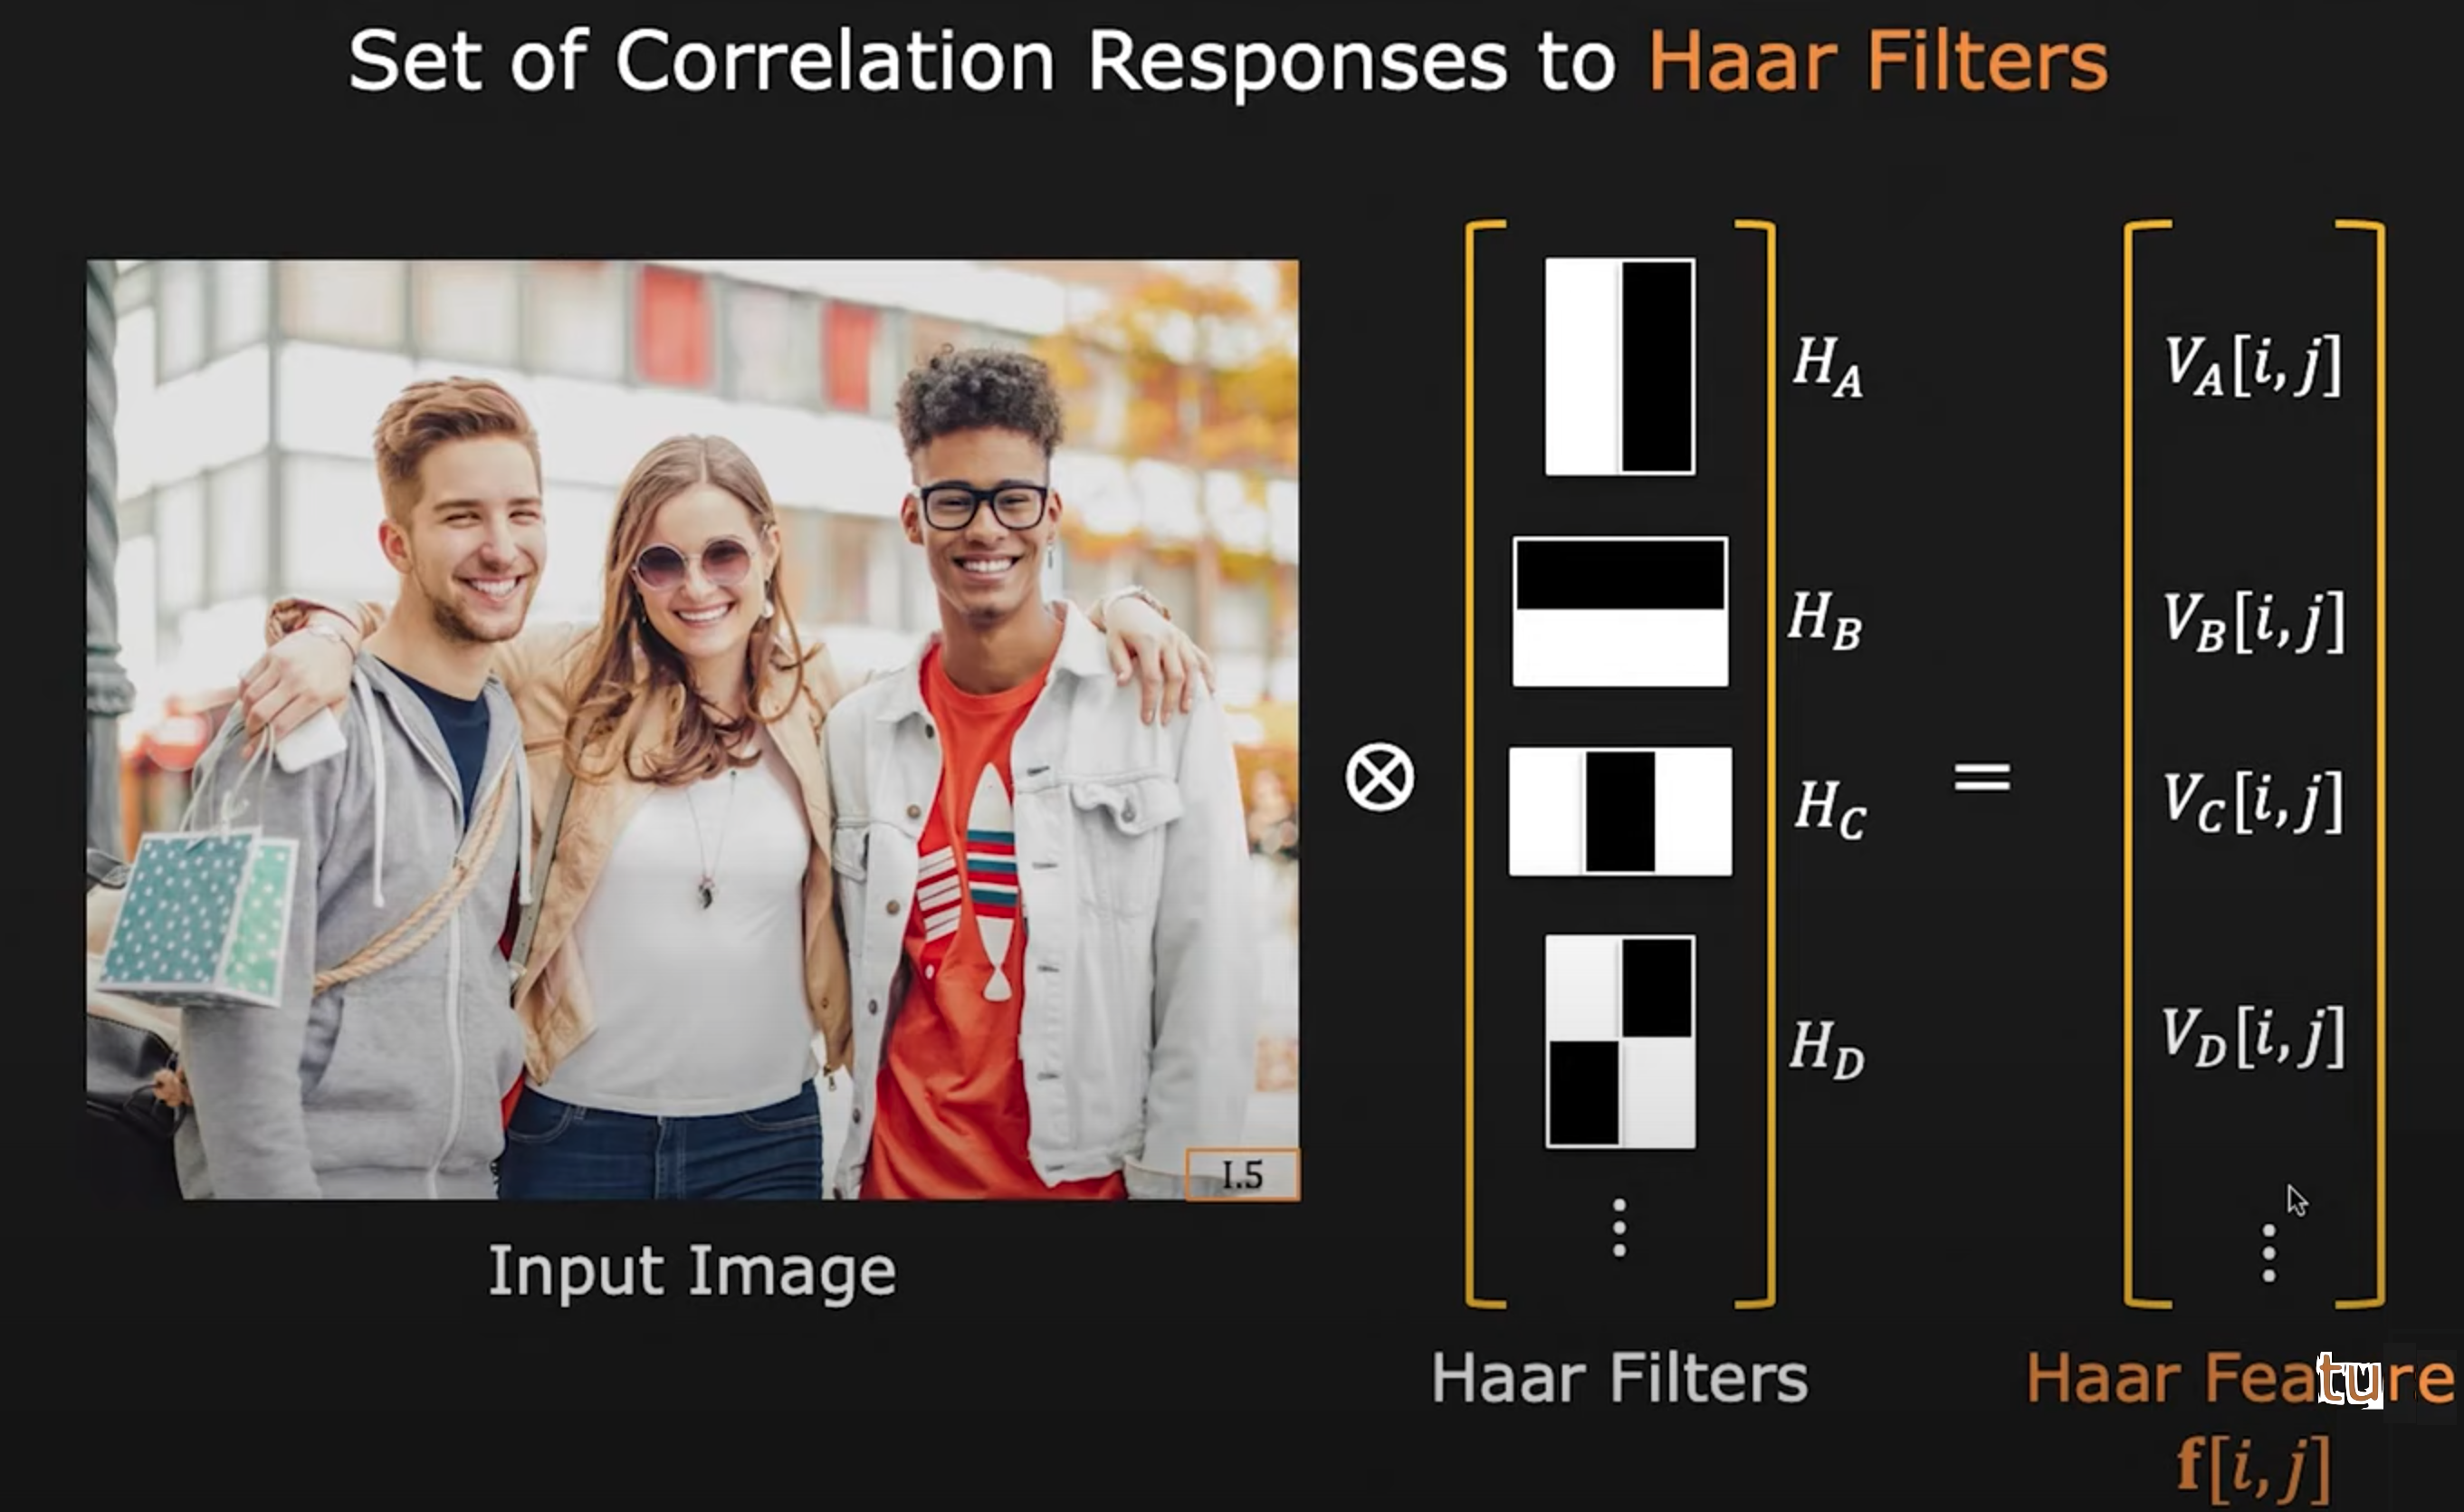
\includegraphics[width=8cm]{images/haar1.png}
  \caption{Discrimination ability of Haar Features}
  \end{figure}
It is based on Haar features, which are computed using Haar filters, two valued filters that make the computations very advantageous. Basically, as it's sketched on the image above, each Haar filters is applied as a correlation on the image and a corresponding value is determined. This value is equivalent to the difference between the sum of the pixels on the white area and sum of the pixels in the black area, as we will see later.
What does an Haar feature do?

\begin{figure} [!hbp]
  \centering
    \begin{subfigure}[b]{0.4\textwidth}
    \centering
    \captionsetup{justification=centering}
      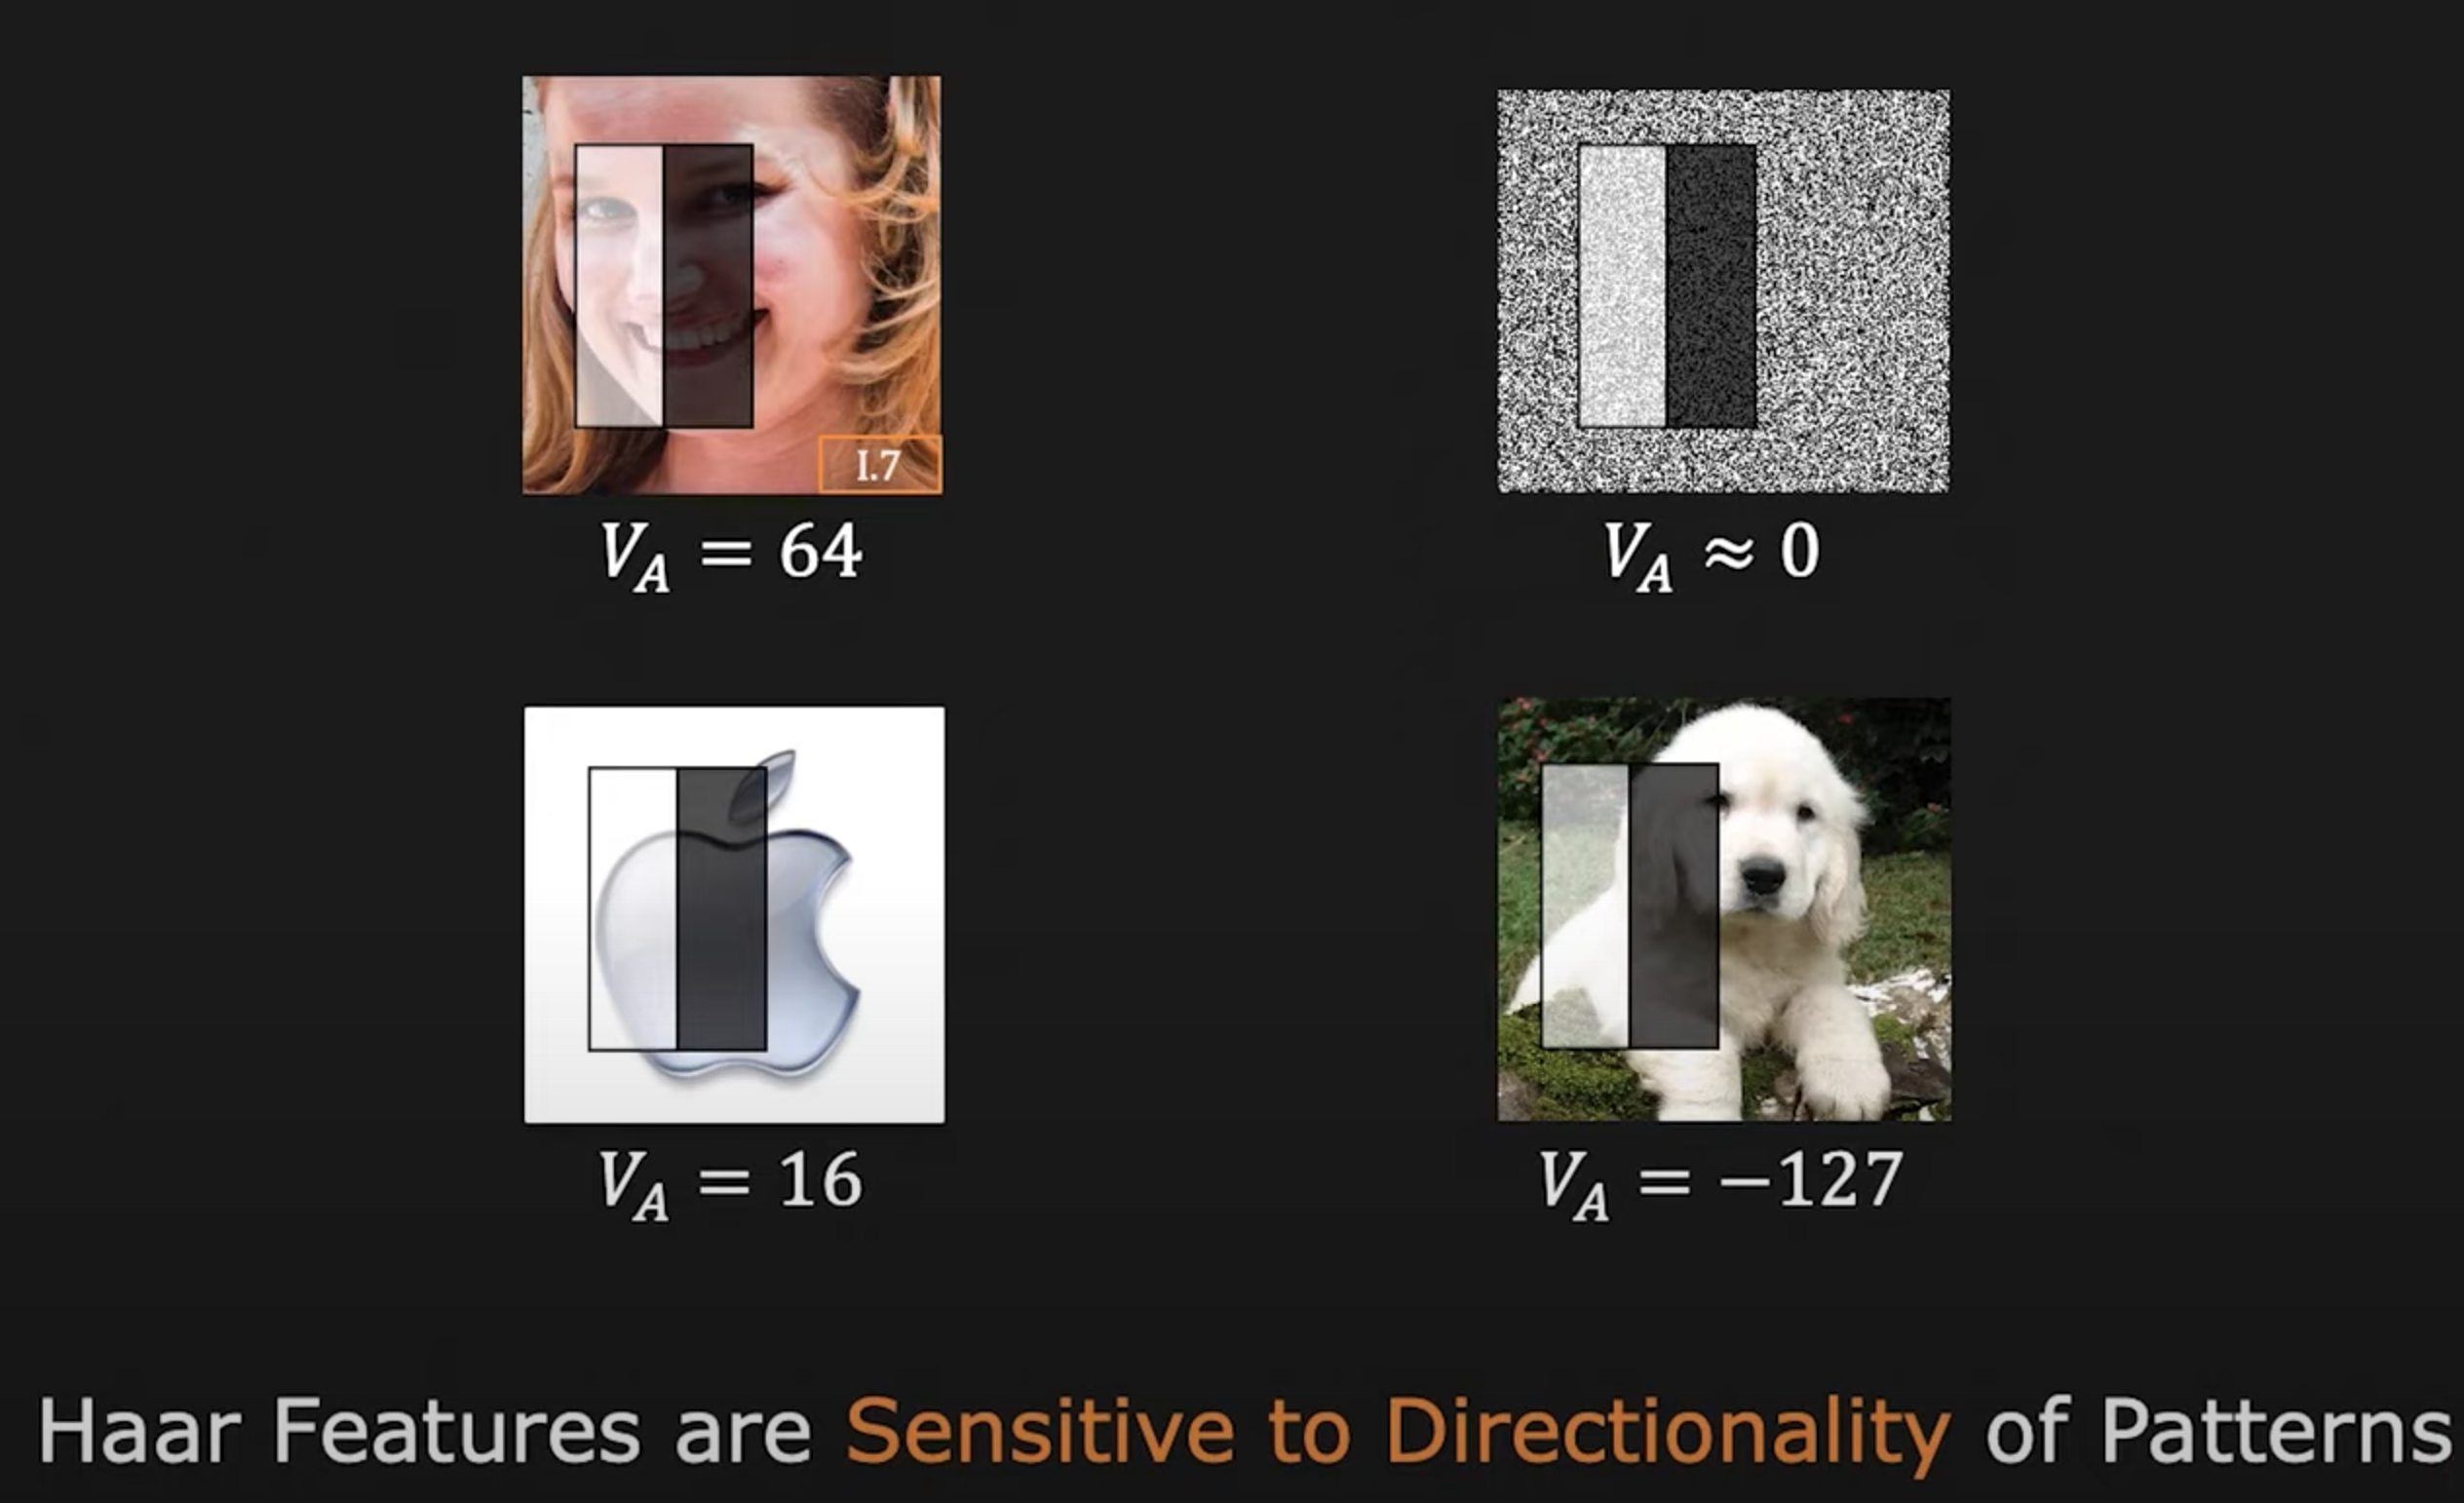
\includegraphics[width=\textwidth]{images/haar2.png}
      \caption{Discrimination ability of Haar Features}
      
    \end{subfigure}
    \hspace{0.1cm}
    \begin{subfigure}[b]{0.4\textwidth}
    \centering
    \captionsetup{justification=centering}
      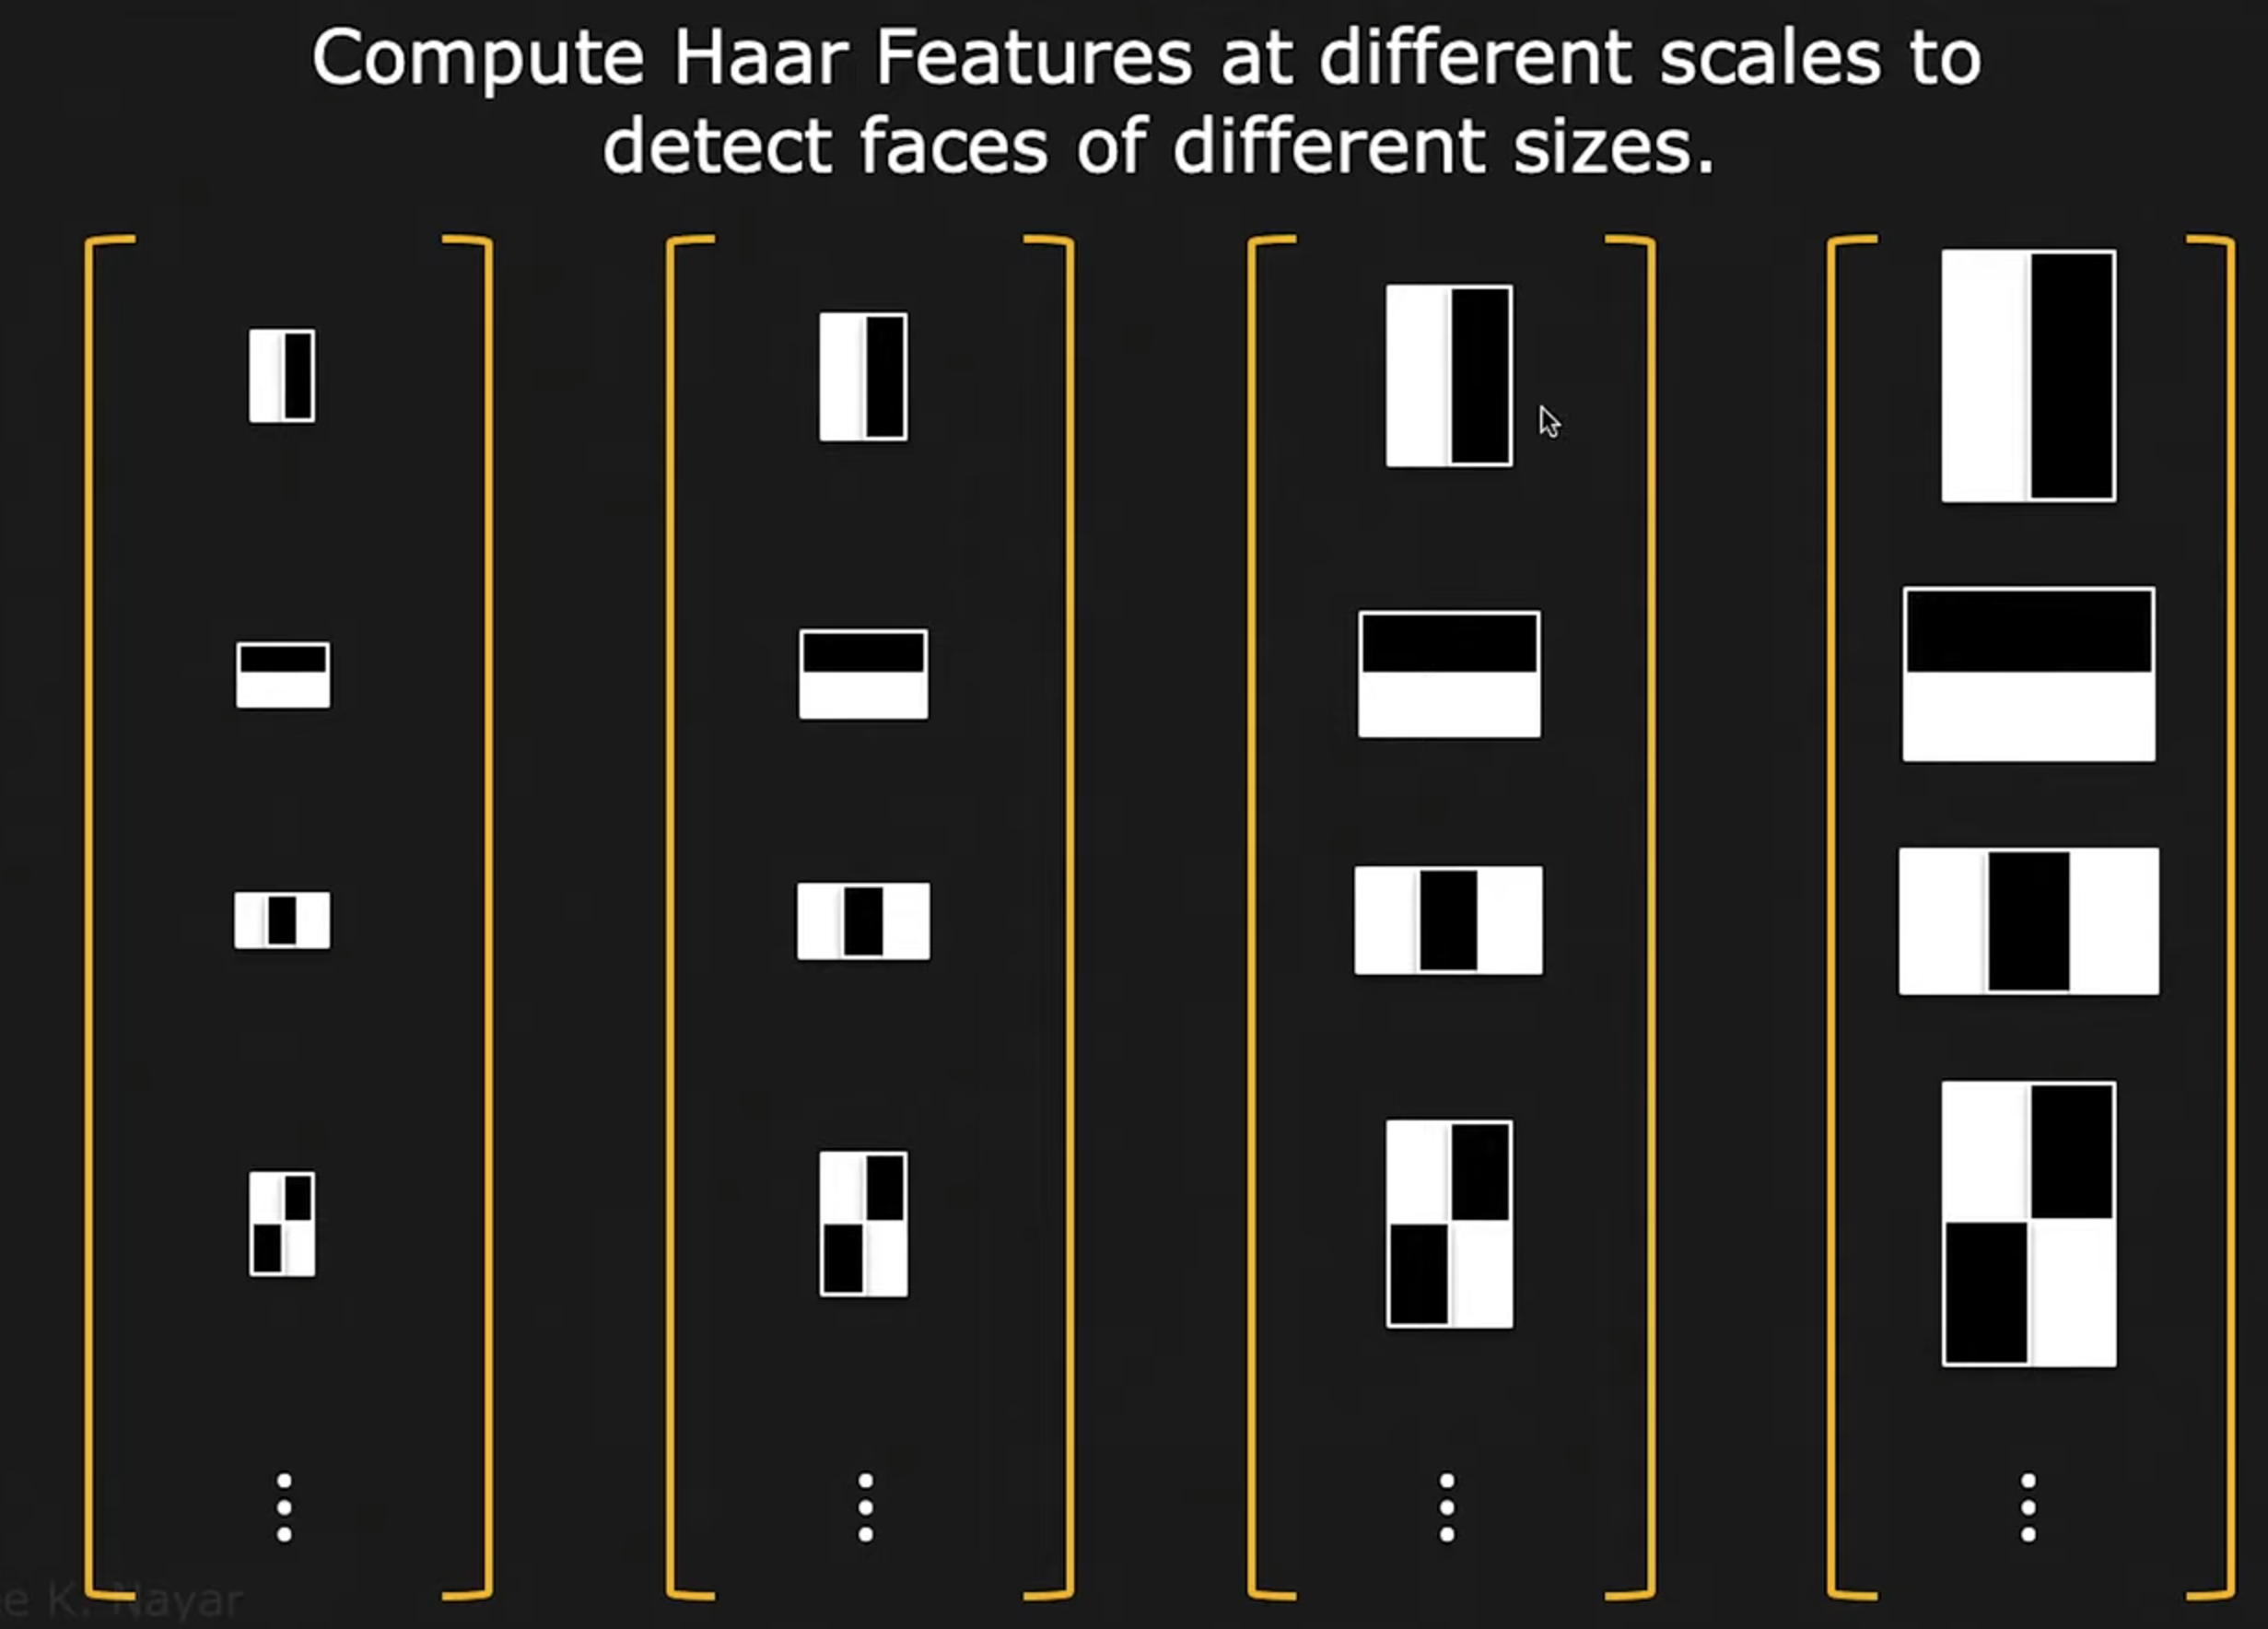
\includegraphics[width=\textwidth]{images/haar3.png}
      \caption{Detecting }
      
    \end{subfigure}
  \end{figure}
Its role consists on detecting differences on intensities on each area where an Haar filter is applied on the image. They are of course sensitive to scale, since if we are scanning an image using a 2 by 2 filter we can't expect to find a face inside. Therefore we're not only going to apply a type of filter while scanning the whole image, but we are also going to apply different scales of the same filter, for a better classification. 
Let's now look at its computational complexity and at how it can be improved.
\begin{figure} [h!]
  \centering
    \begin{subfigure}[b]{0.3\textwidth}
    \centering
    \captionsetup{justification=centering}
      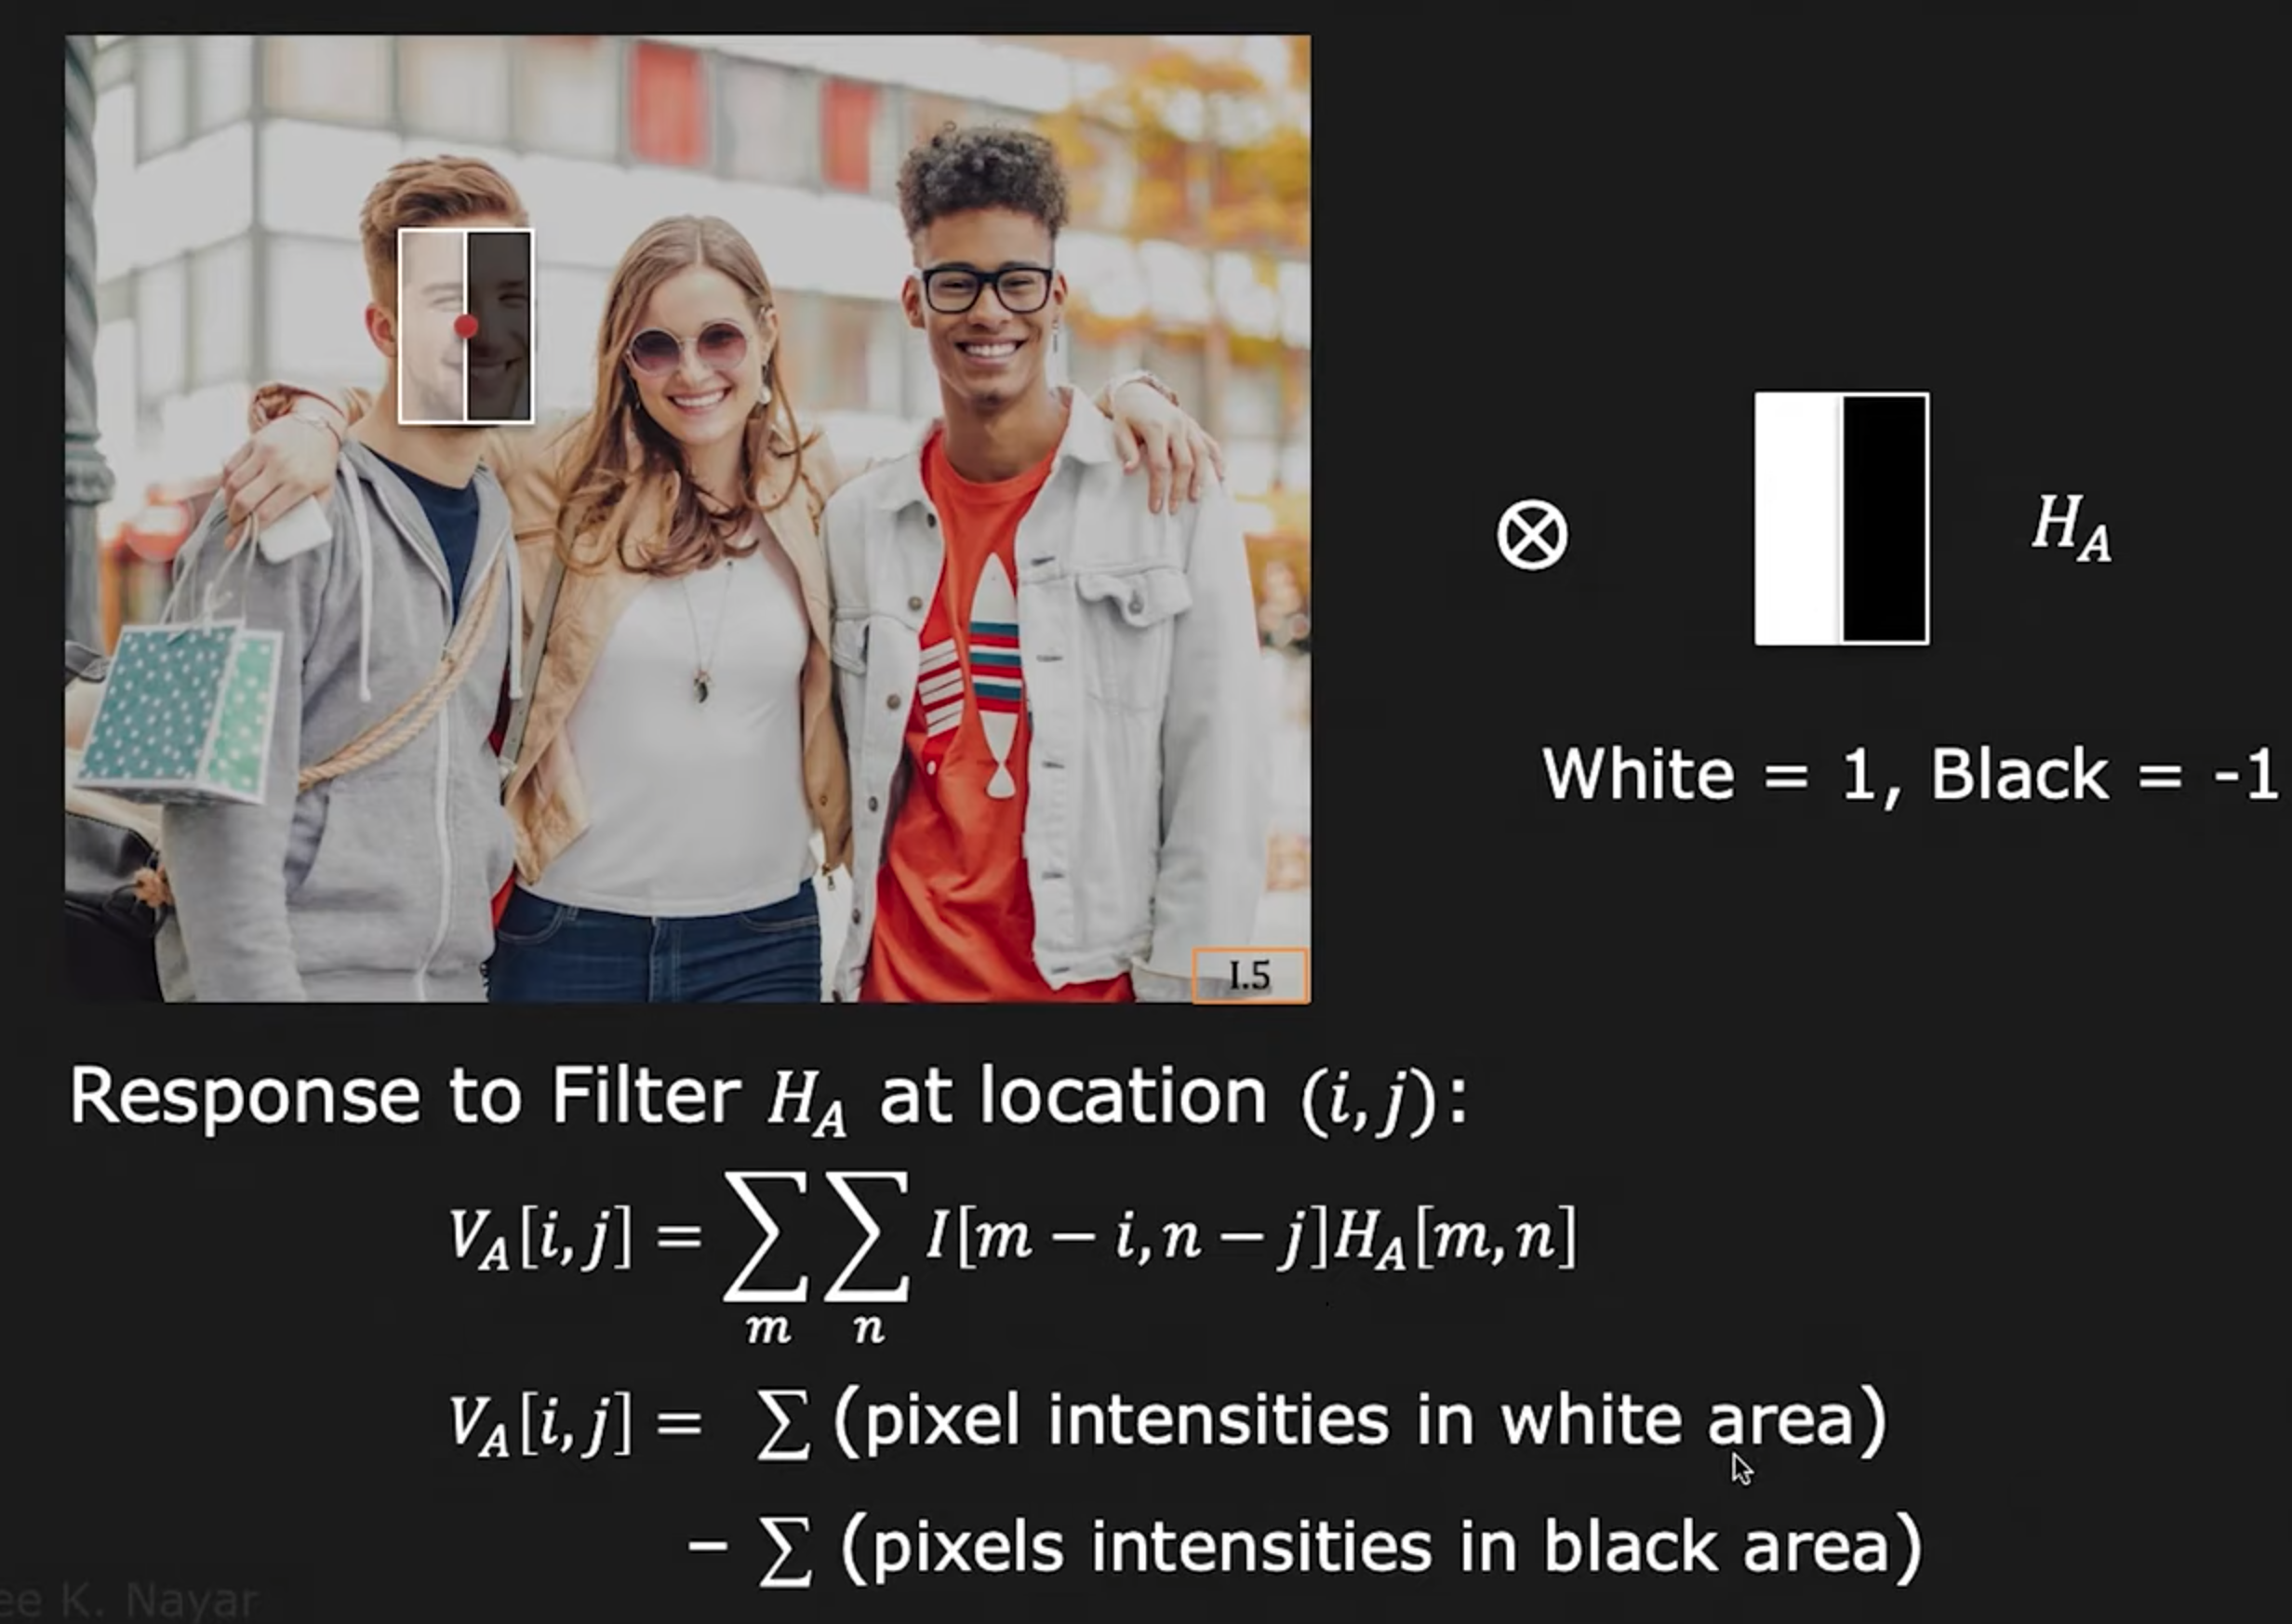
\includegraphics[width=5cm]{images/haar4.png}
      \caption{How to compute an Haar feature}
      
    \end{subfigure}
    \hspace{0.1cm}
    \begin{subfigure}[b]{0.4\textwidth}
    \centering
    \captionsetup{justification=centering}
      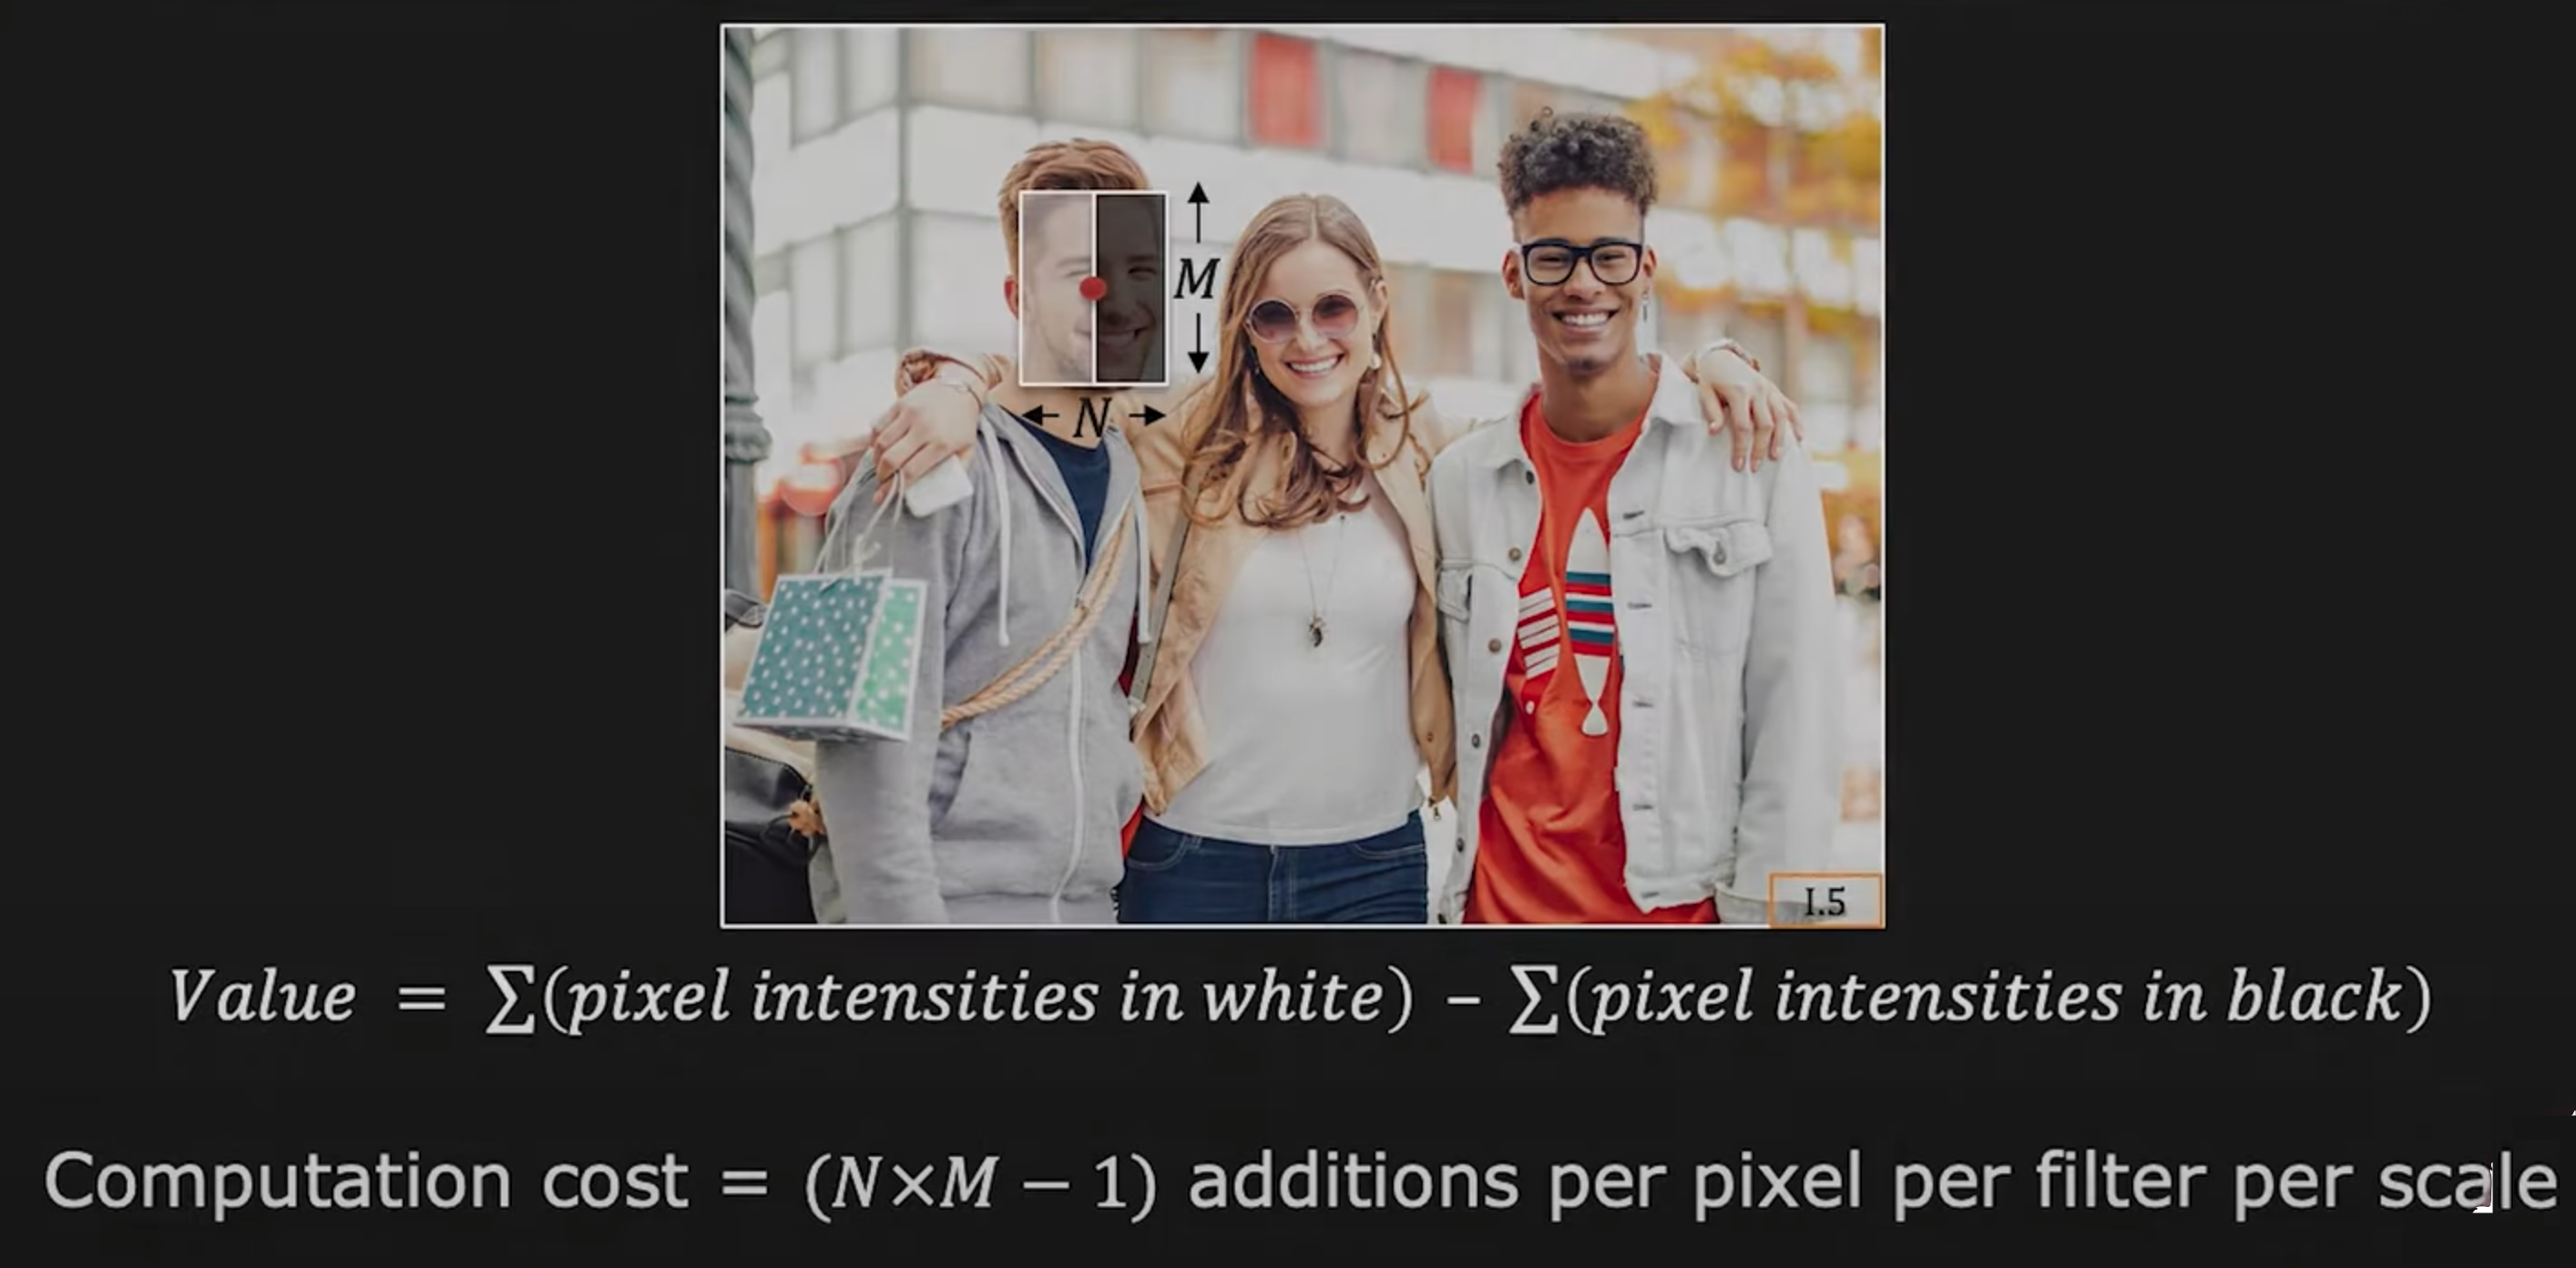
\includegraphics[width=6.5cm]{images/haar5.png}
      \caption{Computational complexity of a single Haar feature}
      
    \end{subfigure}
\end{figure}


As we can see from the image on the left above, an Haar feature is computed by performing the correlation between the Haar filters and the corresponding portion of the image, but since the haar filters are either -1 or 1, we can remove multiplication and only use additions and subtractions, which are a lot cheaper. However, if we have an $M\times N$ filter, we still need to compute $M\times N/2-1$ additions for the two sums and one more for subtracting them, which results in a total of $(N\times M)-1$ of additions per pixel per scaled filter.
This cost can be substantially improved if we use integral images.

\begin{figure} [!h]
  \centering
    \begin{subfigure}[b]{0.4\textwidth}
      \centering
      \captionsetup{justification=centering}
        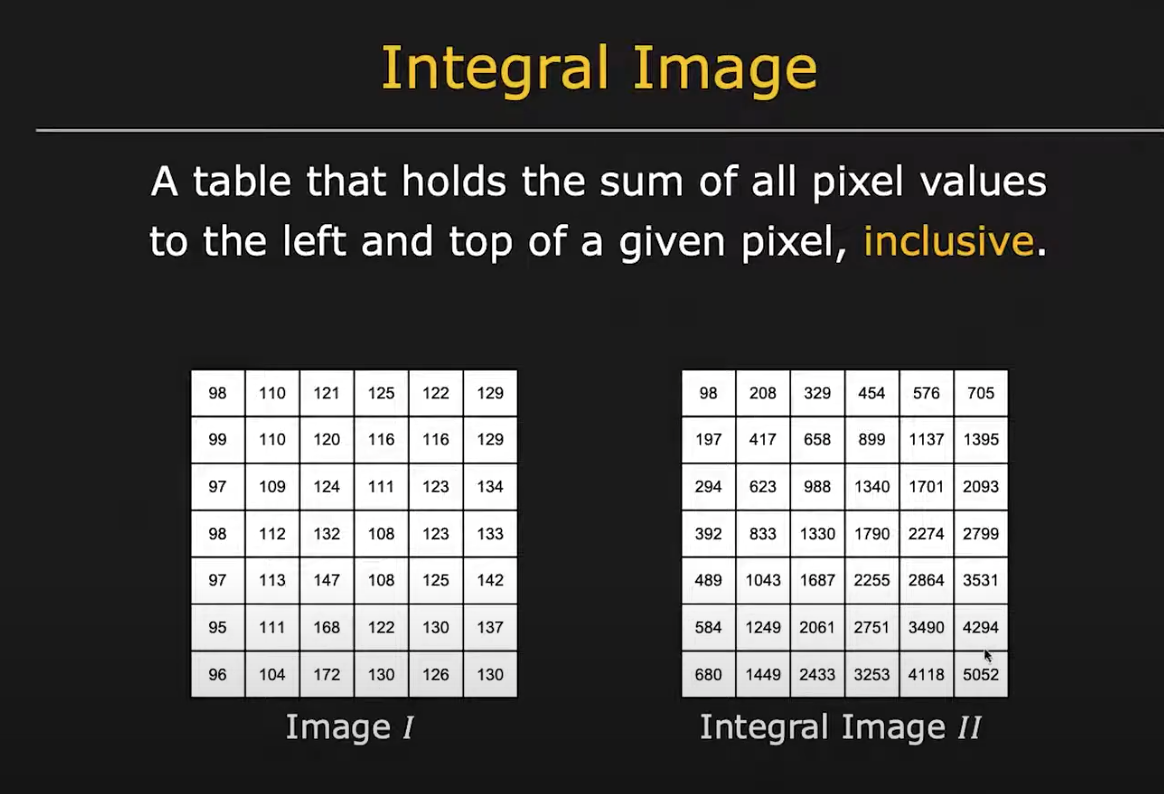
\includegraphics[width=\textwidth]{images/haar6.png}
        \caption{Integral Image}
        
    \end{subfigure}
    \hspace{0.1cm}
    \begin{subfigure}[b]{0.4\textwidth}
      \centering
      \captionsetup{justification=centering}
        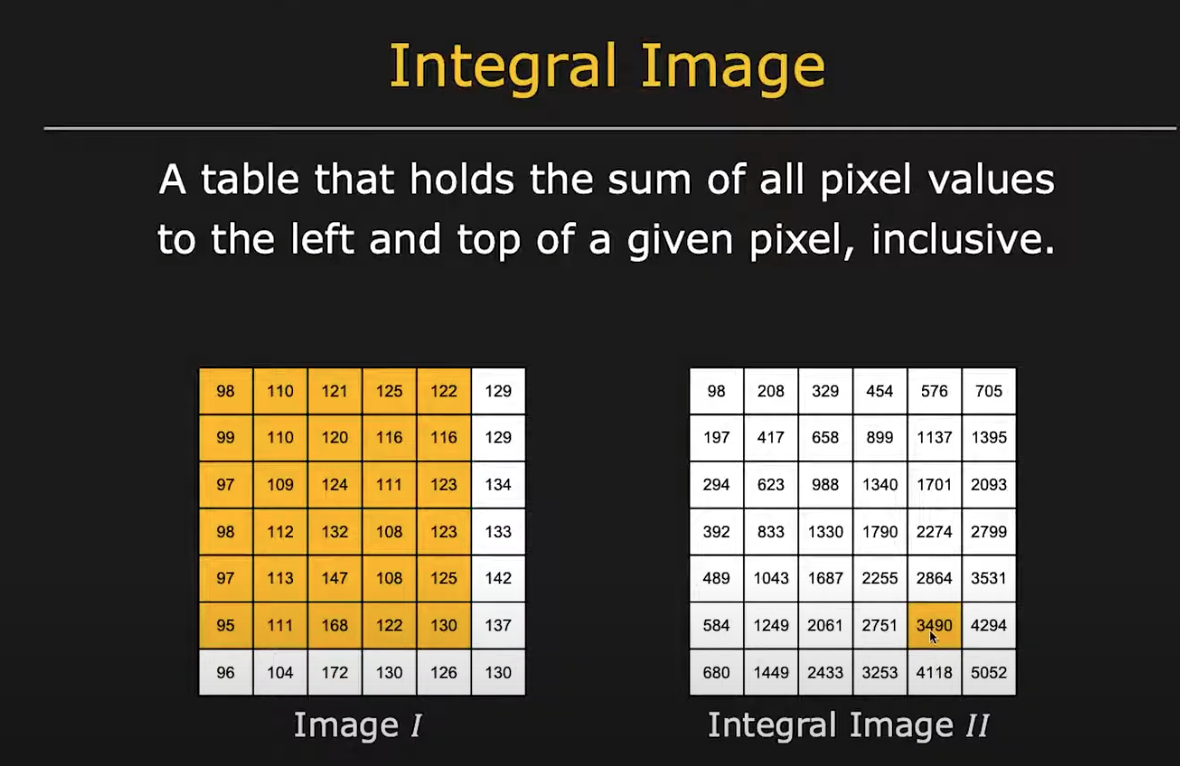
\includegraphics[width=\textwidth]{images/haar7.png}
        \caption{Integral image yellow cell contains sum of all pixels in the yellow rectangle}

      \end{subfigure}
  \end{figure}
These images are tables that pre-store in the bottom right vertex the sum of all the pixels inside each rectangle/square with top left vertex which coincides with the top left one of the image. It can compute the sum of any rectagle using only 3 additions, so for an Haar filter it only need 7 additions.


\begin{figure} [h!]
  \centering
    \begin{subfigure}[b]{0.4\textwidth}
    \centering
    \captionsetup{justification=centering}
      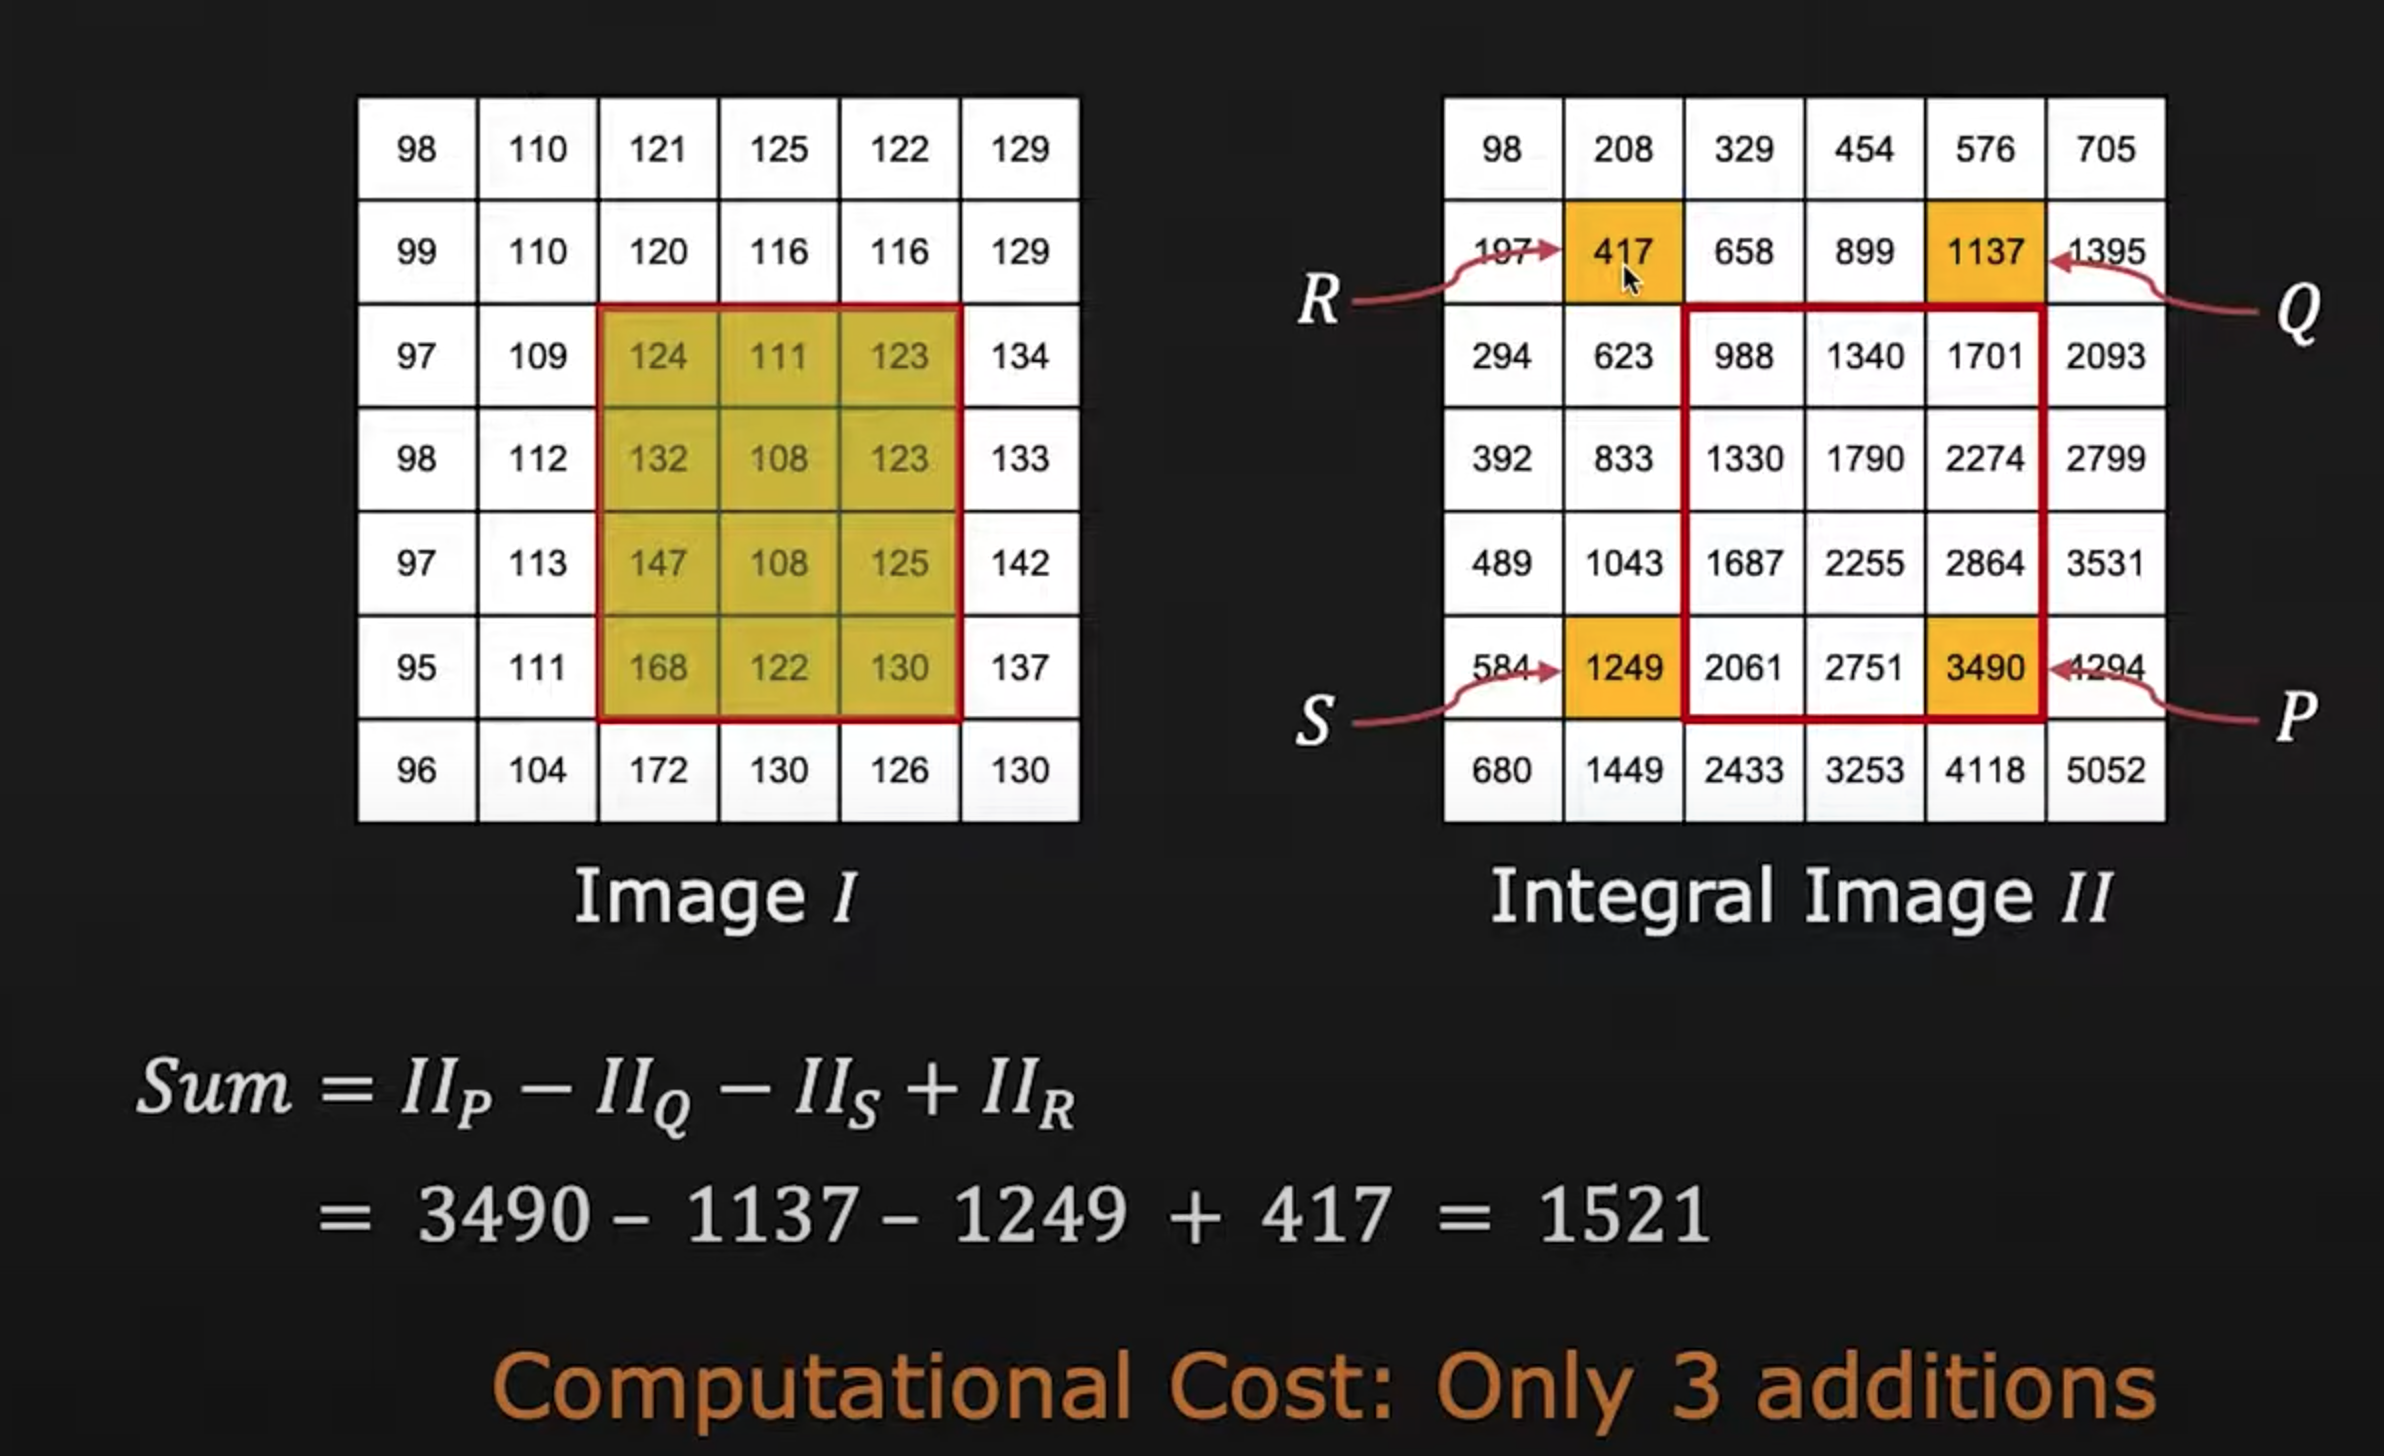
\includegraphics[width=\textwidth]{images/haar8.png}
      \caption{Sum of the pixels in the red square can be computed using only three additions}
      
    \end{subfigure}
    \hspace{0.1cm}
    \begin{subfigure}[b]{0.4\textwidth}
    \centering
    \captionsetup{justification=centering}
      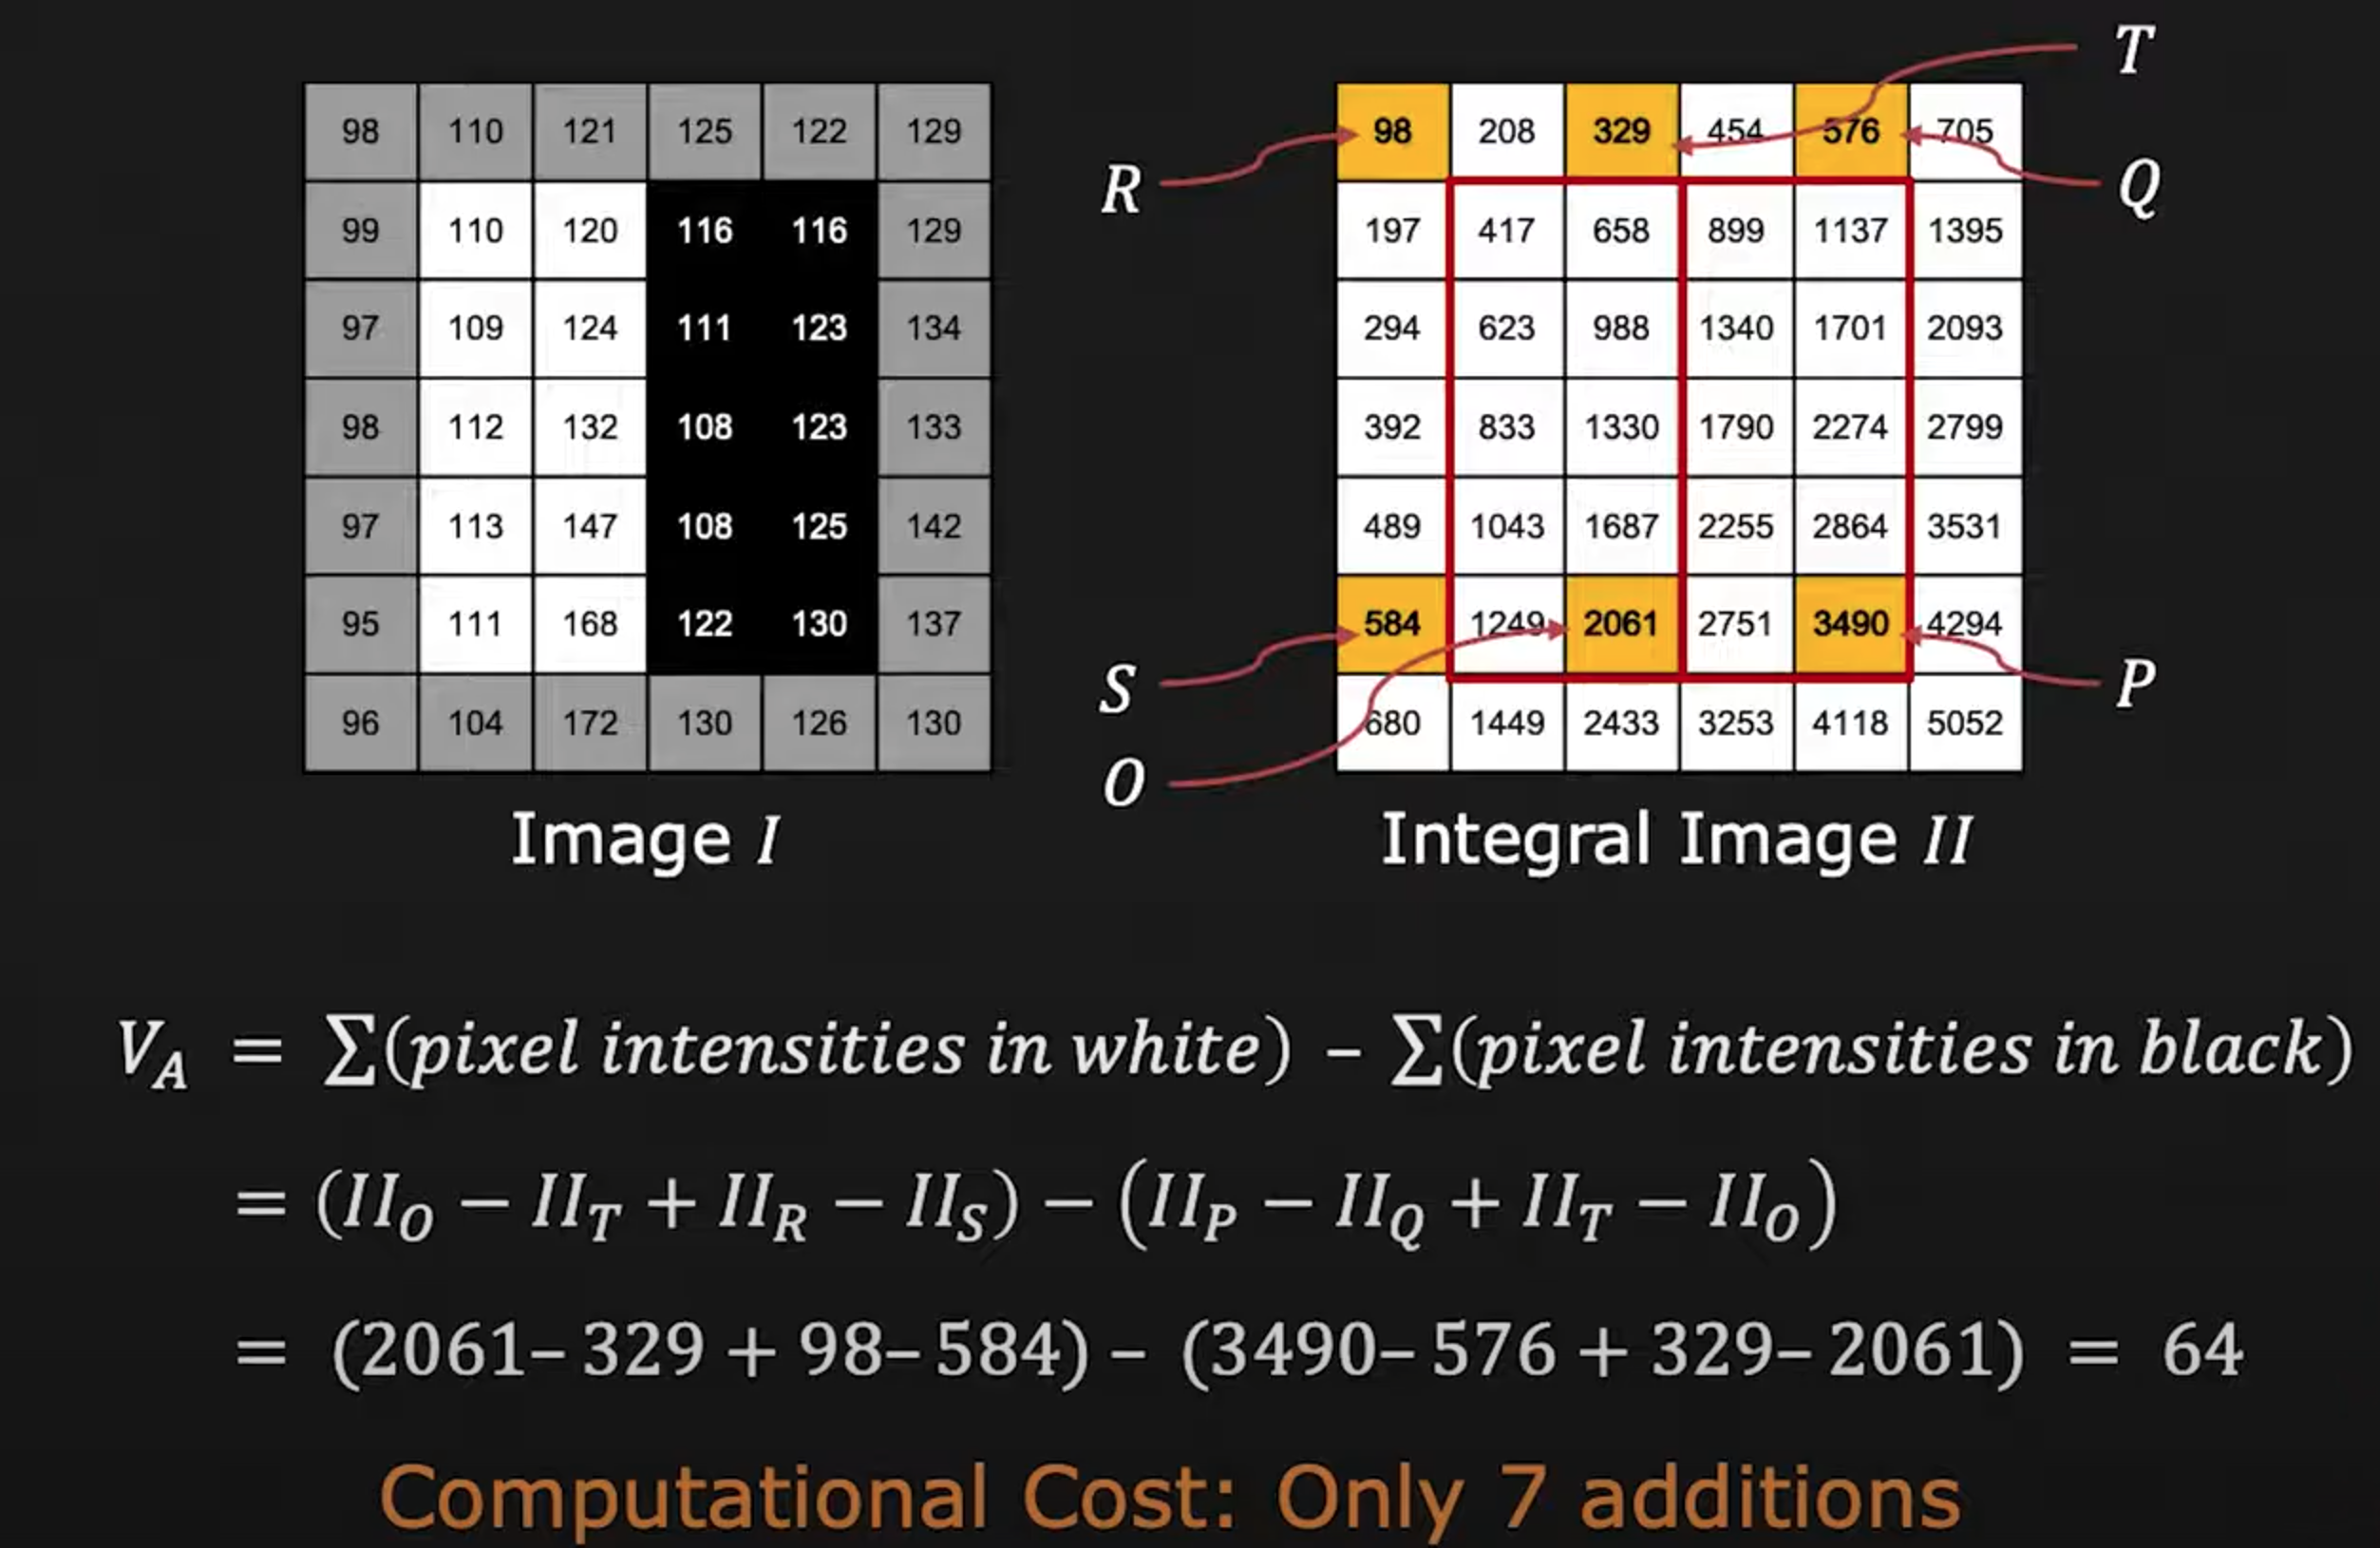
\includegraphics[width=\textwidth]{images/haar9.png}
      \caption{Haar feature can be computed using only 3+3+1=7 additions}
      
    \end{subfigure}
  \end{figure}


It can be processed by simply scanning setting in its pixels the sum of the corresponding cell in the image with the two rectangle above it, represented by the integrals sums B and C in the image below, minus the rectangle D that has been added two times.
\begin{figure} [!h]
  \centering
  \captionsetup{justification=centering}
  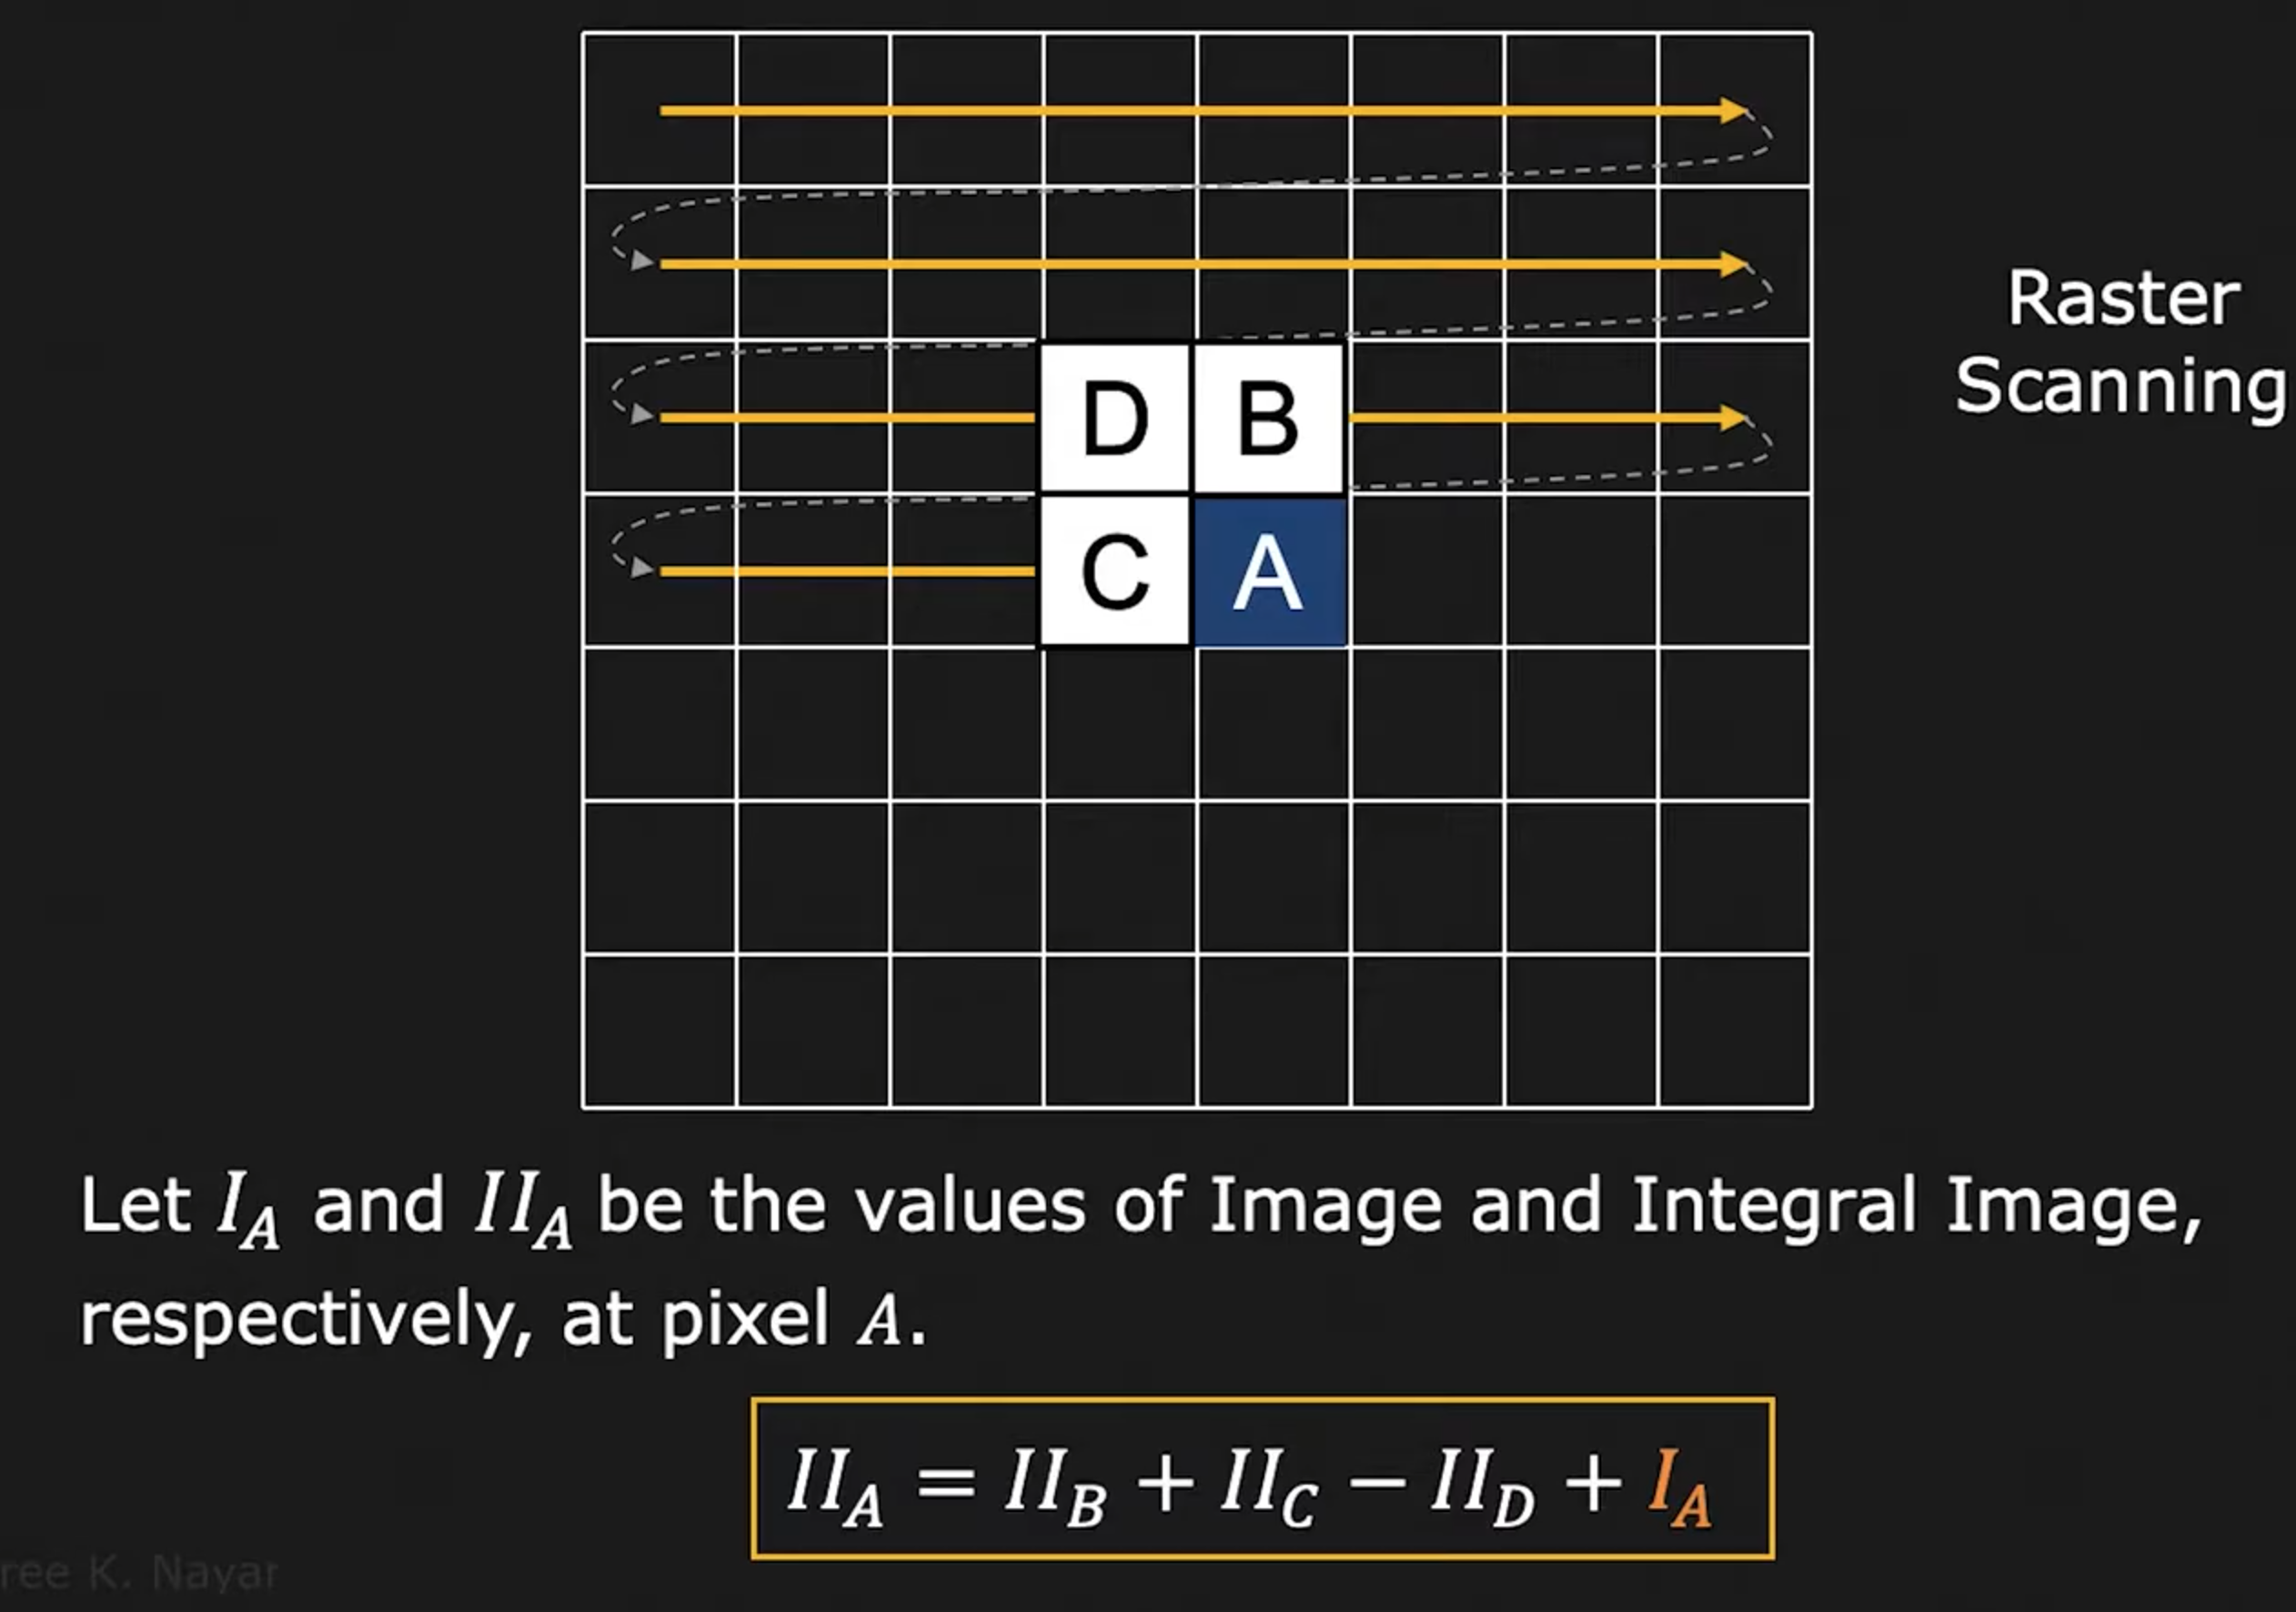
\includegraphics[width=10cm]{images/haar10.png}
  \caption{How to compute the Integral Image}
  \end{figure}

\subsection{Our implementation}
We made a script that extracts images from videos. We made a couple of videos on our 3D printed STOP signals which result in 1700 positive images to give as training set and more or less 2000 negative images as negative samples for the training set. The scripts are on the STOP recognition folder. After setting a couple of hyperparameters, we used \href{https://amin-ahmadi.com/cascade-trainer-gui/}{this GUI} to train the classifier and to speed-up the process, which returned the XML file.
We can now give as input to the Haar cascade classifier implementation of OpenCV our XML file, in order to set the best parameter for detecting the STOPs. Once again, we used trackbars to help us in the selection. We tuned the scale parameter, for selecting the filters with the best scale value; the neig parameter, for removing false positive and only detecting true positives, by considering only window that are in the neighbourhood of other windows; the minArea parameter, since we didn't want very small false positive to be detected; finally, the brightness, in order to be a little more resistant to lightning conditions. Its accuracy is impressive.



\subsection{STOP implementation in our car}
We now know the algorithm that recognizes the sign posts. It returns the position of the top-left bounding box rectangle of the stop signal and its width and height if something is detected, otherwise it returns an emtpy list. Reasonably enough, in order to tell the car that something has been detected we can just verify if the list is empty or not. However in this way, even if the accuracy of our algorithm is pretty high, we're not really sure if that thing that has been detected is a STOP or a false positive. Therefore it would be safer to set a mini-batch that verify that at least the $x$\% of it contains detected frames. And this method works pretty well, it only stops in front of stop posts. But the problem is that it often stops more than once in a row. What I mean is that it detects the sign, it stops and then restart searching for STOP signals and it re-stop. We could change manually the threshold of the number of stops detected, but it's not a smart way of solving the problem, even if it is almost always solved. If it start detecting to late or too early, it can fail to recognize the STOP or halt too far from it. We could make the car move for a certain distance before start searching again for STOP, but then in the improbable case that the sign post is in a curve it will go off-road.
\subsubsection*{Where to STOP}
Therefore the way we managed to solve the problem is by computing the distance from camera to the STOP sign. How do we do that? We will use the "triangle similarity" on the image seen in the camera. As we know, the way an image is formed in the camera follow the same principles of the human eye. Rays of light reflected by the object pass through the lens  from a particular angle and the image is formed in the back side of the wall(the retina, in the case of the human eye). The main difference is that humans have two eyes which receives light at different angles, so they can see the world in three dimensions, while cameras have only one lens, which limits the dimensions to two. But don't worry, we can recover a pretty good estimate of the third distance from the focal length. It is the distance between the camera sensor and the optical center of the camera lens, which is the point where the light rays intercept and it's fixed for each type of lens. It determines the angle of incidence of the light, namely how close an object is from the camera.

\begin{figure} [!h]
  \centering
  \captionsetup{justification=centering}
  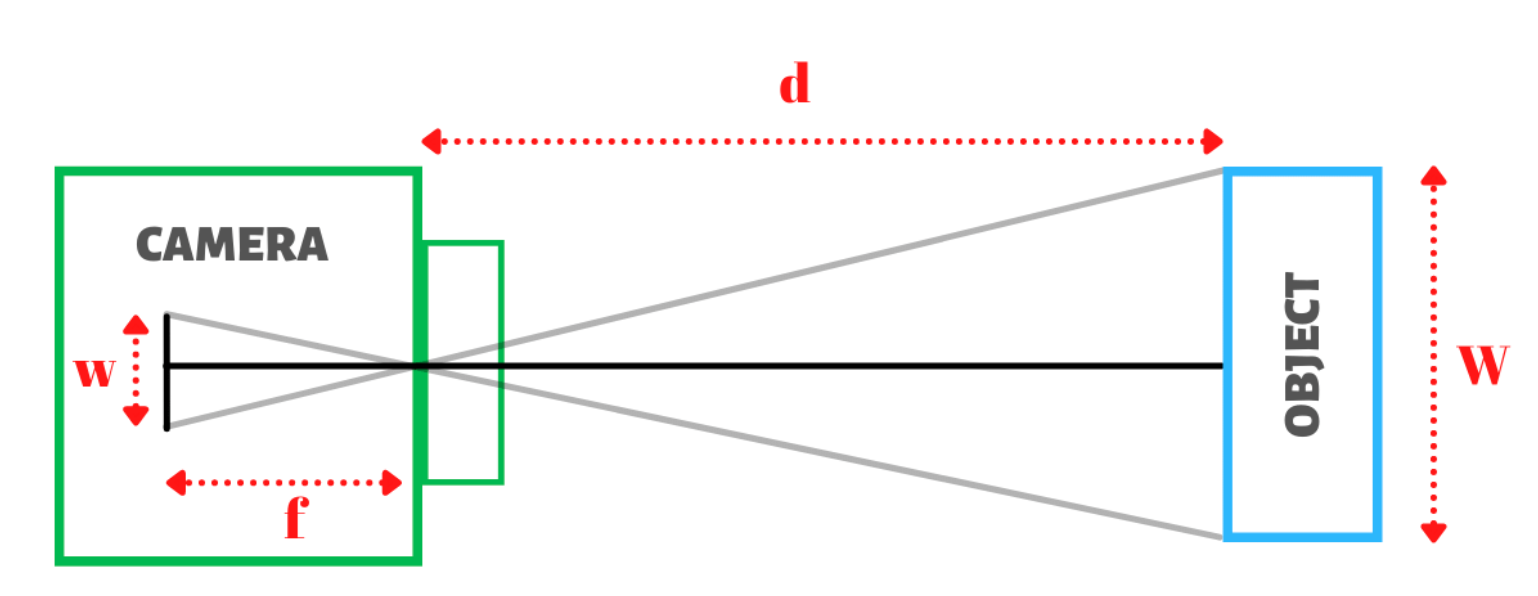
\includegraphics[width=10cm]{images/3D_distance.png}
  \caption{How to determine distance from the camera to an object}
  \end{figure}

Therefore we can see how the width of the STOP seen from the camera is correlated to its real distance from the camera. We can now compute the triangle similarity between the two triangles. Thus the focal length is $f = \frac{w * d}{W}$ and the distance from the object $d = \frac{W * f}{w}$, where $d$ is the focal distance, $w$ the width of the object in the image and $W$ its real length, as you can also see from the image above. We can interpret these results by noting that the focal length and the width of the real object are fixed distances and the smaller an object is in an image, the further it is in the real world. Hence $w*d$ will be always equal to the fixed value $f*D$, for a particular object and a given camera.
So, once found the focal length of the camera by fixing the focal distance of the STOP sign, we can compute the space between them by inserting the width of the perceived image in the formula above, together with the now fixed W and focal length. If the distance from the STOP is between 10cm and 15cm, the car stops, in all other cases go straight.


\section{Conclusion}
After building the vehicle and preparing the path, having written the code for the image processing lane detection and having tested it multiple times,  we can officially say that we manage to build a self-driving car which is able to predict the trajectory to take and is able to STOP in proximity of a STOP signal, almost like a real autonomous vehicle! \\


\section{Self-Evaluation $\&$ Future Projects}
We can say with utmost certainty that the takeaway from a project like this is definitely going to help in the future. Having designed an autonomous vehicle we feel equipped with the tools to learn more about Computer Vision and we are heading to further improve this project next year during the deep learning course, by implementing the lane detection with Neural Networks and by adding more knowledge tothe world, like our beloved semaphore recognition and pedestrian detection. We could also add vocal command during the NLP course, by simply telling it order with our voice. We can basically add any sort of things to make the project cooler and we can't wait to improve it further. Indeed, a project like this will be a great learning experience just like our final project was. \\

\section{References}
\begin{itemize}
\item[1] Thresholding - OpenCV - Documentation\\ \url{https://docs.opencv.org/4.x/d7/d4d/tutorial_py_thresholding.html}
\item[2] Warp perspective - OpenCV - Documentation\\
\url{https://docs.opencv.org/4.x/da/d54/group__imgproc__transform.html}
\item[3] Color spaces - OpenCV - Documentation\\
\url{https://docs.opencv.org/4.x/df/d9d/tutorial_py_colorspaces.html}
\item[4]  Focal length | Youtube and links on Code \\
\url{https://www.youtube.com/watch?v=4CoEsqePADw}
\item[5] Haar features - Wikipedia, the free encyclopedia\\
\url{https://en.wikipedia.org/wiki/Haar-like_feature}
\item[6] Haar Cascade - Columbia University\\
\url{https://fpcv.cs.columbia.edu}
\item[7] Viola-Jones Algorithm - Rapid Object Detection using a Boosted Cascade of Simple Features\\
\url{https://www.cs.cmu.edu/~efros/courses/LBMV07/Papers/viola-cvpr-01.pdf}
\end{itemize}

\noindent\rule{18.5cm}{0.4pt}
\end{large} 
\end{document}
